% =====================================================================
% ClubMS --  Project Report
% ---------------------------------------------------------------------
% Compile with: pdflatex -> pdflatex (run twice for ToC/LoF/LoT/refs)
% Requires a standard TeX Live / MiKTeX installation (tikz, booktabs,
% tabularx, titlesec, setspace, hyperref, enumitem, caption, float).
%
% All screenshot figures are marked with a boxed placeholder so the
% author can drop in real screenshots later. Diagrams (architecture,
% ERD, sequence, state, deployment) are generated directly in TikZ.
%
% Edit the fields in the "REPORT META-DATA" block below before
% compiling the cover page.
% =====================================================================
\documentclass[12pt,oneside]{book}

% ---------------------------------------------------------------------
% Packages
% ---------------------------------------------------------------------
\usepackage[a4paper,left=1.5in,right=1in,top=1in,bottom=1in]{geometry}
\usepackage[T1]{fontenc}
\usepackage[utf8]{inputenc}
\usepackage{times}                 % Times New Roman substitute (Nimbus Roman)
% --- If you prefer the exact Times New Roman font and compile with
%     XeLaTeX/LuaLaTeX instead, comment out "times" above and use:
% \usepackage{fontspec}
% \setmainfont{Times New Roman}
\usepackage{setspace}
\usepackage{titlesec}
\usepackage{graphicx}
\usepackage{caption}
\usepackage{tabularx}
\usepackage{booktabs}
\usepackage{longtable}
\usepackage{array}
\usepackage{multirow}
\usepackage{enumitem}
\usepackage{xcolor}
\usepackage{float}
\usepackage{tikz}
\usetikzlibrary{arrows.meta,positioning,shapes.geometric,calc}
\usepackage[hidelinks]{hyperref}
\urlstyle{same}
\usepackage{microtype}



% ---------------------------------------------------------------------
% Spacing
% ---------------------------------------------------------------------
\setlength{\parindent}{0.3in}
\onehalfspacing
\tolerance=1000
\emergencystretch=2em
\hbadness=10000

% ---------------------------------------------------------------------
% Caption formatting: centered, bold label
% ---------------------------------------------------------------------
\captionsetup{justification=centering, labelfont=bf, font=small, singlelinecheck=false}
\captionsetup[table]{position=top}
\captionsetup[figure]{position=bottom}

% ---------------------------------------------------------------------
% Chapter / heading formatting
%   Chapter titles : Times New Roman, 16pt, CAPS, BOLD
%   Headings       : Times New Roman, 14pt, bold
%   Sub-headings   : Times New Roman, 12pt, bold
% ---------------------------------------------------------------------
\titleformat{\chapter}[display]
  {\centering}
  {\bfseries\fontsize{14}{16}\selectfont \MakeUppercase{\chaptertitlename}\ \thechapter}
  {8pt}
  {\bfseries\fontsize{16}{19}\selectfont\MakeUppercase}
\titlespacing*{\chapter}{0pt}{10pt}{25pt}

\titleformat{\section}
  {\normalfont\fontsize{14}{16}\selectfont\bfseries}{\thesection}{1em}{}
\titleformat{\subsection}
  {\normalfont\fontsize{12}{14}\selectfont\bfseries}{\thesubsection}{1em}{}
\titleformat{\subsubsection}
  {\normalfont\fontsize{12}{14}\selectfont\bfseries\itshape}{\thesubsubsection}{1em}{}

% ---------------------------------------------------------------------
% Page style
% ---------------------------------------------------------------------
\pagestyle{plain}

% ---------------------------------------------------------------------
% Reusable TikZ styles for diagrams
% ---------------------------------------------------------------------
\tikzset{
  ent/.style={draw, thick, rectangle, rounded corners=2pt, align=center, minimum width=2.6cm, minimum height=1cm, font=\small, fill=gray!7},
  proc/.style={draw, thick, rectangle, rounded corners=2pt, align=center, minimum width=3.4cm, minimum height=1.1cm, font=\small, fill=gray!7},
  hl/.style={draw, thick, rectangle, rounded corners=2pt, align=center, minimum width=3.4cm, minimum height=1.1cm, font=\small, fill=black!10},
  st/.style={draw, thick, ellipse, align=center, minimum width=3.6cm, minimum height=1.3cm, text width=3cm, font=\small, fill=gray!7},
  arr/.style={-{Stealth[length=2.2mm]}, thick},
  darr/.style={-{Stealth[length=2.2mm]}, thick, dashed},
  lbl/.style={font=\tiny, align=center}
}

% ---------------------------------------------------------------------
% Screenshot placeholder helper
% ---------------------------------------------------------------------
\newcommand{\screenshotbox}[1]{%
  \fbox{\begin{minipage}[c][#1][c]{0.85\textwidth}
    \centering\itshape Insert Figure here
  \end{minipage}}%
}
\newcommand{\FigurePlaceholder}[3]{%
\begin{figure}[H]
\centering
\screenshotbox{#1}
\caption{#2}
\label{#3}
\end{figure}
}
\newcommand{\ScreenshotFigure}[3]{%
\begin{figure}[H]
\centering
\includegraphics[width=\textwidth,keepaspectratio]{#1}
\caption{#2}
\label{#3}
\end{figure}
}
\usepackage{booktabs}
\usepackage{tabularx}
\usepackage{float}
\usepackage{array}
\usepackage{ragged2e}
\newcolumntype{L}[1]{>{\RaggedRight\arraybackslash}p{#1}}
\begin{document}

% =====================================================================
% COVER PAGE
% =====================================================================
\begin{titlepage}
\thispagestyle{empty}
\centering

\vspace*{0.3cm}
{\fontsize{20}{24}\selectfont\bfseries UNIVERSITY CLUB MANAGEMENT}\\[0.3cm]
{\fontsize{20}{24}\selectfont\bfseries PLATFORM (ClubMS)}

\vspace{0.9cm}
{\fontsize{18}{22}\selectfont\bfseries B.Sc. Level 3 Semester II PROJECT REPORT}\\[0.2cm]
{\fontsize{18}{22}\selectfont\bfseries Course Code: CSE 352}\\[0.2cm]
{\fontsize{18}{22}\selectfont\bfseries Course Title: Web and Mobile Application Development Sessional}

\vspace{0.9cm}
{\fontsize{16}{19}\selectfont\bfseries Prepared by}

\vspace{0.3cm}
{\fontsize{14}{17}\selectfont
\begin{tabular}{@{}c@{}}
Md Farhan Quadery \\
ID: 2202015 \\[0.3cm]
Md Saddam Hosen Molla \\
ID: 2202042 \\
\end{tabular}
}

\vspace{3cm}

\IfFileExists{hstu-logo.png}{%
  
\includegraphics[width=4cm,height=4cm]{hstu-logo.png}%
\begin{figure}
    \centering
    
\includegraphics[width=0.5\linewidth]{hstu-logo.png}
    \caption{Enter Caption}
    \label{fig:placeholder}
\end{figure}
}{%
  \fbox{\begin{minipage}[c][4cm][c]{4cm}\centering\itshape University Logo\end{minipage}}%
}

\vspace{0.9cm}
{\fontsize{18}{22}\selectfont\bfseries Department of Computer Science and Engineering}\\[0.15cm]
{\fontsize{14}{17}\selectfont\bfseries Hajee Mohammad Danesh Science and Technology University,}\\[0.1cm]
{\fontsize{14}{17}\selectfont\bfseries Dinajpur-5200}

\end{titlepage}
\pagenumbering{roman}

% =====================================================================
% ABSTRACT
% =====================================================================
\chapter*{ABSTRACT}
\addcontentsline{toc}{chapter}{ABSTRACT}

Most universities still run their student clubs on paper forms, spreadsheets, and WhatsApp groups, or else pay for closed, subscription-based engagement suites that cannot be self-hosted or customized. ClubMS was built to close that gap: a self-hosted, white-label club management platform with a Node.js/Express/Prisma REST API on PostgreSQL and a React frontend (Vite, Tailwind, Radix UI). It supports four roles -- Platform Admin, Club Admin, Faculty, and Student -- under a layered authorization model that checks both global role and per-resource ownership. On top of that sit a full club and membership lifecycle with department-based join rules and a join-agreement flow; multi-club events run through a consent-based co-host invitation system; RSVP tracking; announcements; a venue directory; magic-byte-validated file uploads for logos, banners, and ID cards; and an audit log for accountability. The whole system runs on Docker Compose and can be rebranded for any institution just by changing a few environment variables. Built over about five months, it is backed by 345 automated tests -- both unit tests and full HTTP integration tests run against a real, disposable PostgreSQL instance via Testcontainers. This report covers the motivation behind the project, how it compares to existing academic and commercial club-management systems, the requirements gathered from three user groups, the design and implementation, the results, a cost comparison against commercial alternatives, and where the project falls short and could be extended.

\vspace{0.5cm}
\noindent\textbf{Keywords:} club management system, role-based access control, white-label web application, React, Node.js.

% =====================================================================
% TABLE OF CONTENTS / LIST OF FIGURES / LIST OF TABLES
% =====================================================================
\tableofcontents
\listoffigures
\listoftables

% =====================================================================
% MAIN MATTER
% =====================================================================
\mainmatter

% #####################################################################
\chapter{Introduction}
% #####################################################################

\section{Background}

Student clubs and societies are a core part of campus life: they give students a structured way to build skills, form communities, and engage with campus activities outside the classroom. Running them, however, generates a steady stream of administrative work -- accepting or rejecting membership applications, tracking who is an active member versus an alumnus, scheduling and publicizing events, recording attendance, and keeping an auditable trail of decisions such as promotions and removals.

In many institutions this work is still done manually. A 2017 case study of the Student Affairs Department at Universiti Teknologi MARA, Terengganu found that club registration and event-proposal processing were handled through paper forms and repeated manual re-entry every semester, motivating the development of a dedicated online club management system [1]. More recent student projects report the same pattern in a different guise: a 2025 case study of club coordination at D. Y. Patil College of Engineering and Technology found that roughly twenty clubs relied on individual WhatsApp groups for communication, leading to fragmented, hard-to-audit information flow [2]. Where institutions do invest in dedicated software, the market is dominated by large, closed, subscription-priced campus-engagement suites such as CampusGroups and Modern Campus Involve (formerly Presence), which bundle orientation management, gamified badging, ticketing, and analytics into a single vendor-hosted product [3]. These products are capable, but they are licensed per institution or per student, cannot be self-hosted, and offer little control over branding, data residency, or the underlying data model.

ClubMS was built to occupy the space between these two extremes: a system that is as structured and auditable as a purpose-built platform, but that a university (or a single department) can deploy on its own infrastructure, brand with its own name, logo, and color, and extend without being tied to a vendor's roadmap or pricing.

\begin{figure}[H]
\centering
\resizebox{\textwidth}{!}{%
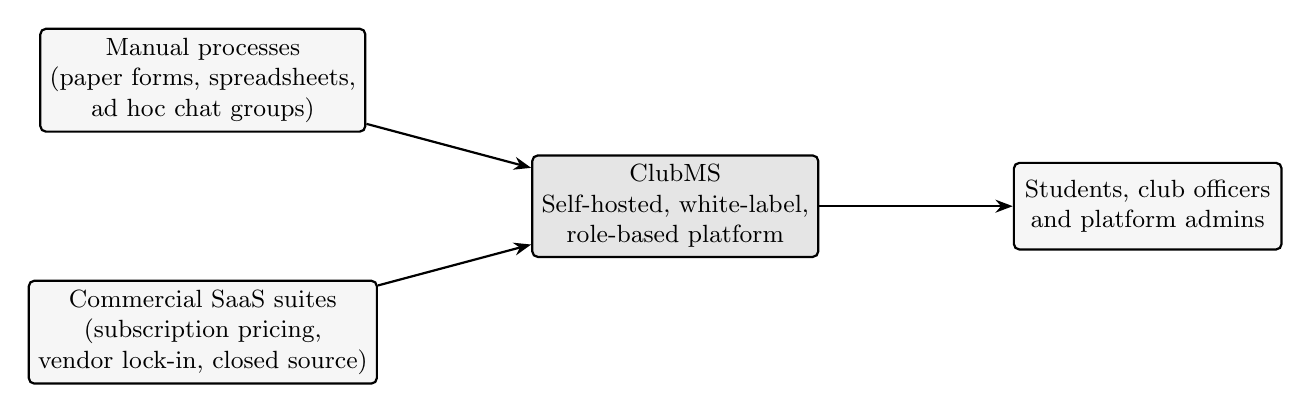
\begin{tikzpicture}
\node[proc] (manual) at (0,1.6) {Manual processes\\(paper forms, spreadsheets,\\ad hoc chat groups)};
\node[proc] (saas) at (0,-1.6) {Commercial SaaS suites\\(subscription pricing,\\vendor lock-in, closed source)};
\node[hl] (clubms) at (6,0) {ClubMS\\Self-hosted, white-label,\\role-based platform};
\node[proc] (users) at (12,0) {Students, club officers\\and platform admins};
\draw[arr] (manual) -- (clubms);
\draw[arr] (saas) -- (clubms);
\draw[arr] (clubms) -- (users);
\end{tikzpicture}%
}
\caption{Conceptual positioning of ClubMS between manual coordination methods and commercial SaaS platforms}
\label{fig:1.1}
\end{figure}

\section{Problem Statement}

Three recurring problems motivate this project:

\begin{enumerate}[label=(\alph*)]
\item \textbf{Manual, error-prone administration.} Paper-based or spreadsheet-based membership and event tracking does not scale past a handful of clubs, is difficult to audit, and gives no structured way to enforce eligibility rules (for example, restricting membership to particular departments) or to track the lifecycle of a request from submission to approval [1].
\item \textbf{Fragmented, unaccountable communication.} Ad hoc tools such as WhatsApp groups and shared spreadsheets provide no persistent, role-aware record of who requested to join a club, who approved it, who hosted an event, or who attended it [2].
\item \textbf{Vendor lock-in and cost of commercial alternatives.} Existing dedicated platforms are commercially licensed, closed-source, hosted exclusively by the vendor, and priced in a way that is often out of reach for smaller institutions, individual departments, or student-run initiatives, while offering no meaningful way to self-host or white-label the product [3].
\end{enumerate}

There is a clear need for a system that gives institutions the structure and accountability of a dedicated platform while remaining self-hostable, inspectable, and brandable at no licensing cost.

\section{Motivation}

The motivation for this project is both practical and technical. Practically, the author observed the same administrative friction described above in the context of student club coordination, where officers had no systematic way to manage pending join requests, promote members to officer roles, or coordinate events that involve more than one club. Technically, it was a chance to design and build a production-grade, full-stack system end-to-end rather than a classroom-scale demo. That meant a normalized relational schema that grew through eighteen incremental migrations, an authorization model robust enough to resist both blunt mistakes (a missing role check) and subtler ones (a missing per-resource ownership check), a componentized and accessible frontend, a test suite that hits real HTTP endpoints against a real database instead of mocked collaborators, and a deployment pipeline a real university could actually adopt without much setup.

\section{Objectives}

\subsection{General Objective}
To design, implement, and evaluate a self-hosted, white-label web-based club management platform that digitizes the full lifecycle of university clubs, memberships, and events for three primary user groups (four system roles).

\subsection{Specific Objectives}
\begin{enumerate}
\item To design a relational data model and REST API that represent clubs, memberships, events, RSVPs, announcements, and administrative audit trails.
\item To implement a role-based access control (RBAC) system with role inheritance and per-resource ownership checks that scale from a single-club officer to a platform administrator.
\item Implement a complete club and membership lifecycle, including department-based join eligibility rules, a join-agreement flow, and bulk moderation tools for officers.
\item To implement an event management module that supports a single primary host club and a consent-based invitation workflow for co-hosting events across clubs.
\item To implement secure file upload handling (club logos, event banners, and student ID cards) that validates file content rather than trusting client-supplied metadata.
\item To implement a white-labeling mechanism that allows an institution's brand color, logo, and name to be configured without modifying application code.
\item To validate the system with an automated test suite covering both isolated utility functions and full HTTP integration paths against a real database.
\item To package the system for reproducible deployment using Docker and Docker Compose.
\end{enumerate}


% #####################################################################
\chapter{Related Work}
% #####################################################################

\section{Overview}

Club and society management is a well-studied problem in student capstone and applied-research literature, and it is also served by a mature commercial market of campus-engagement platforms. This chapter reviews six representative works -- five academic projects and one category of commercial products -- and positions ClubMS against them. Table~\ref{tab:2.1} summarizes each work bibliographically; Table~\ref{tab:2.2} compares their features, strengths, and weaknesses relative to the objectives of this project.



\begin{table}[H]
\caption{Bibliographic summary of related club/society management systems}
\label{tab:2.1}
\centering
\small
\begin{tabularx}{\textwidth}{@{}L{0.5cm}L{3cm}L{5cm}>{\RaggedRight\arraybackslash}X@{}}
\toprule
\# & Author(s) / Year & Title & Platform / Technology \\
\midrule
{[1]} & Syd. Amra (2017) & Online Club Management System for UiTM Terengganu (On-ClubS) & PHP/MySQL intranet web system; SDLC with Extreme Programming \\
{[4]} & Kumar et al. (2025) & Club Management System: A MERN Stack-Based Web Application for Event Management in Colleges & MongoDB, Express, React, Node.js (MERN) \\
{[5]} & Nath et al. (2025) & College Club Management System -- Digitizing Student Engagement and Organizational Efficiency & HTML/CSS/JavaScript, Node.js, MySQL, Power BI (framework proposal) \\
{[2]} & Ainapure et al. (2025) & DYPCETCLUBS -- A Unified Platform for Management of College Clubs & React, TypeScript, Tailwind CSS; Node.js, Express; SQLite with Prisma ORM \\
{[6]} & Qi (2024) & Design and Implementation of University Club Management System based on WeChat Applet & WeChat Mini Program (JavaScript) with cloud database \\
{[3]} & Modern Campus / CampusGroups (commercial) & Campus engagement platforms (CampusGroups; Modern Campus Involve, formerly Presence) & Proprietary, vendor-hosted SaaS \\
\bottomrule
\end{tabularx}
\end{table}

\section{On-ClubS -- UiTM Terengganu (2017)}
On-ClubS automated the Student Affairs Department's paper-based workflow for approving new club proposals and event proposals at a single campus [1]. It was built using a conventional PHP/MySQL stack and evaluated with a usability questionnaire that reported generally positive results. Its scope, however, stops at the proposal-approval stage: it does not model ongoing membership status, does not expose a student-facing join/browse experience, and includes no concept of roles beyond staff versus student. It also targets a single institution's server and has no branding or multi-deployment story.

\section{MERN-Stack Club Management System (2025)}
This paper presents a club and event management system built on the MERN stack (MongoDB, Express, React, Node.js) that automates event scheduling, authentication, participation tracking, and real-time notifications, and explicitly cites role-based access control as a design goal [4]. It is architecturally close to ClubMS's frontend/backend split, but the published work does not describe a membership lifecycle with distinct pending/active/alumni/rejected states, does not address multi-club event collaboration, and does not discuss deployment, white-labeling, or automated testing.

\section{College Club Management System -- Framework Proposal (2025)}
This work is a survey- and literature-driven proposal for a ``College Club Management System'' rather than a fully implemented product; it enumerates the problems of manual club administration and sketches a target feature set based on stakeholder interviews [5]. It is included here because it independently corroborates the problem statement in Chapter~1 -- fragmented communication and manual processes -- but, being a proposal, it offers no working implementation, authorization model, or evaluation to compare directly against ClubMS.

\section{DYPCETCLUBS (2025)}
DYPCETCLUBS is notable for using a technology stack very close to ClubMS's: React with TypeScript and Tailwind CSS on the frontend, and Node.js/Express with Prisma ORM on the backend [2]. It centralizes event management, notifications, and recruitment for roughly twenty college clubs that previously relied on WhatsApp groups. Its main limitations relative to ClubMS are its use of SQLite (a single-writer, file-based database not well suited to concurrent multi-club production use), the absence of a documented role-inheritance model or per-resource authorization layer, and no mention of containerized deployment, white-labeling, audit logging, or a consent-based cross-club collaboration workflow.

\section{WeChat Applet Club Management System (2024)}
This system reimplements club management as a WeChat Mini Program backed by a cloud database, aiming to increase interactivity by meeting students inside an app they already use [6]. While effective for institutions where WeChat is the dominant platform, the design is inherently locked to the WeChat ecosystem: it is not accessible as an ordinary web application, has no independent admin dashboard, and cannot be self-hosted or white-labeled outside of WeChat's own infrastructure.

\section{Commercial Campus Engagement Suites}
Platforms such as CampusGroups and Modern Campus Involve are mature, feature-rich SaaS products offering orientation management, virtual involvement fairs, gamified badging, integrated budgeting and payments, and analytics dashboards for large institutions [3]. They are the strongest systems in this comparison in terms of breadth of features and production maturity. Their weaknesses, from the perspective of this project's objectives, are structural rather than functional: they are closed-source, licensed on a recurring commercial basis, hosted exclusively by the vendor (no self-hosting option), and offer only theming-level customization rather than control over the underlying codebase or data model.

\section{Gap Analysis}

\begin{table}[H]
\caption{Feature comparison between related systems and ClubMS}
\label{tab:2.2}
\centering
\small
\begin{tabularx}{\textwidth}{@{}p{2.6cm}X X@{}}
\toprule
System & Strengths & Weaknesses relative to ClubMS \\
\midrule
On-ClubS [1] & Automates paper-based proposal workflow; evaluated with real users & No membership lifecycle, no RBAC hierarchy, single-institution, no self-service join flow \\
MERN CMS [4] & Modern JS stack; RBAC and notifications cited as goals & No documented multi-status membership lifecycle, no multi-club events, no test suite discussed \\
College CMS proposal [5] & Grounded in stakeholder research; validates the problem statement & Proposal only -- no working implementation to compare \\
DYPCETCLUBS [2] & Near-identical tech stack (React/Tailwind, Node/Express/Prisma) & SQLite (not production-scale), no audit trail, no cross-club collaboration, not white-label \\
WeChat Applet CMS [6] & High reach within WeChat-native user base & Locked to WeChat platform; not self-hostable or brandable \\
Commercial suites [3] & Very broad feature set; proven at scale & Closed-source, subscription-priced, vendor-hosted only, no white-label deployment \\
\midrule
\textbf{ClubMS} & \multicolumn{2}{p{9.5cm}}{Self-hosted via Docker Compose; white-labeled at build time; four-role RBAC with inheritance \emph{and} per-resource ownership checks; full PENDING/ACTIVE/ALUMNI/REJECTED membership lifecycle; department-based join rules and join-agreement gating; consent-based cross-club event co-hosting; magic-byte-validated uploads; full audit trail; 345-case automated test suite with a real database} \\
\bottomrule
\end{tabularx}
\end{table}

None of the six systems reviewed here combine self-hosted deployment, white-label branding, a layered RBAC model, consent-based multi-club collaboration, and an integration test suite that runs against a real database. That combination is where ClubMS sits.


% #####################################################################
\chapter{Requirement Specifications}
% #####################################################################

\section{Stakeholders and User Roles}

ClubMS serves three primary human stakeholder groups, mapped onto four system roles (Faculty is a superset of Student and Club Admin permissions, used for faculty advisors who also moderate clubs).

\begin{table}[H]
\caption{System roles and their primary concerns}
\label{tab:3.1}
\centering
\small
\begin{tabularx}{\textwidth}{@{}p{2.6cm}X@{}}
\toprule
Role & Primary concerns \\
\midrule
Student & Discover and join clubs, browse and RSVP to events, manage their own profile, view club announcements. \\
Club Admin (Officer) & Approve or reject membership requests, promote/demote members, manage events for clubs they officer, post announcements, configure join rules. \\
Faculty & Advises one or more clubs; inherits Club Admin and Student permissions for the clubs they are associated with. \\
Platform Admin & University IT / student-affairs staff. Creates and deletes clubs, manages the venue directory, reviews the platform-wide audit log, and has administrative access across all clubs. \\
\bottomrule
\end{tabularx}
\end{table}

\section{Stakeholder Consultation and Field Interviews}
\label{sec:3.2}

Alongside the literature and product review in Chapter~2, the requirements in this chapter were also shaped directly by informal, in-person interviews with sitting officers of four active student organizations at Hajee Mohammad Danesh Science and Technology University (HSTU). The goal was to ground the feature set in problems that real club officers were currently experiencing, rather than relying solely on assumptions carried over from the reviewed systems. Table~\ref{tab:3.1a} lists the club officers consulted.

\begin{table}[H]
\caption{Club officers consulted during requirements gathering}
\label{tab:3.1a}
\centering
\small
\begin{tabularx}{\textwidth}{@{}L{5.4cm}L{4.3cm}X@{}}
\toprule
Club / Organization & Name & Position \\
\midrule
CSE Club of HSTU & Eusha Sarwar Utal & Vice President \\
Programmers Arena & Md. Shohag Showdagor; Kh. Ishtiak Muntasir & Vice President; General Secretary \\
HSTU Football Club & Nur Ahmed Tonmoy; Samiul Huda Juwel & Assistant Vice President; Registrar \\
Tangail District Students' Welfare Association-HSTU & Md. Emon Mahabub Emu & Vice President \\
\bottomrule
\end{tabularx}
\end{table}

\subsection{Interview Approach}

Each interview was conducted face-to-face on campus and followed a short, semi-structured format lasting roughly 20--30 minutes: officers were first asked to walk through how their club currently handled membership intake, event coordination, and record keeping, and were then asked what a digital system would need to support for them to actually adopt it over their existing workflow. Notes were taken during each conversation and later cross-checked against the officer's own description of their process. The recurring pain points raised in these conversations, and how each was ultimately addressed in ClubMS, are summarized in Table~\ref{tab:3.1b}.

\begin{table}[H]
\caption{Problems reported by club officers and the corresponding ClubMS solution}
\label{tab:3.1b}
\centering
\small
\begin{tabularx}{\textwidth}{@{}L{3.4cm}X L{4.7cm}@{}}
\toprule
Reported by & Problem & ClubMS solution \\
\midrule
CSE Club of HSTU (Eusha Sarwar Utal) & Membership applications came in through a Google Form and were approved manually from a spreadsheet; there was no way to tell an applicant their request was still pending, and no record of who approved a given member or when. & Structured membership requests with a visible \texttt{PENDING} state and officer-only approve/reject actions (FR-7, FR-8), each recorded in the audit log with the approving officer and timestamp (FR-20). \\
Programmers Arena (Md. Shohag Showdagor, Kh. Ishtiak Muntasir) & Recruitment was open to the whole university even though the club's charter restricts general membership to CSE students, which the officers had no way to enforce except by manually rejecting ineligible applicants after the fact; joint contests with the CSE Club also had no clean way to show both clubs as organizers on one event. & Department-based join-rule configuration that evaluates eligibility automatically at request time (FR-6, FR-7), and a consent-based co-host invitation workflow so a second club can be added as an official event organizer only after its own officer accepts (FR-12, FR-13). \\
HSTU Football Club (Nur Ahmed Tonmoy, Samiul Huda Juwel) & Attendance for practice sessions and matches was tracked on paper, and building an eligible-player roster for tournament registration meant retyping names from that paper list into a form by hand. & Per-event RSVP tracking with an officer-visible attendee list (FR-15, FR-16) and one-click CSV export of the club roster (FR-10). \\
Tangail District Students' Welfare Association-HSTU (Md. Emon Mahabub Emu) & Announcements were posted in a WhatsApp group, where older messages quickly scrolled out of view and new members had no way to see the association's history of past notices or club rules. & A persistent, pinnable club announcements panel visible to all members (FR-17) and published club rules text shown to prospective members during the join flow (FR-7). \\
\bottomrule
\end{tabularx}
\end{table}

\subsection{Representative Interview Excerpts}

The exchanges below are paraphrased summaries of the interview conversations, included to illustrate the kind of day-to-day friction that motivated the corresponding features.

\medskip
\noindent\textbf{Eusha Sarwar Utal, Vice President, CSE Club of HSTU}

\smallskip
\noindent\textbf{Q:} How does someone currently join the CSE Club?

\noindent\textbf{A:} They fill out a Google Form, and one of us copies the responses into a spreadsheet and messages them once we've decided. It works, but if three of us are handling forms that week, sometimes the same person gets approved twice or nobody follows up at all.

\smallskip
\noindent\textbf{Q:} What would make you trust a digital system to replace that?

\noindent\textbf{A:} Mainly that it shows the request is still pending instead of the student just messaging us to ask, and that it keeps a record of who approved who -- right now if there's a dispute about a membership, nobody can prove what actually happened.

\bigskip
\noindent\textbf{Md. Shohag Showdagor, Vice President \& Kh. Ishtiak Muntasir, General Secretary, Programmers Arena}

\smallskip
\noindent\textbf{Q:} Is membership open to everyone, or restricted?

\noindent\textbf{A (Showdagor):} It's open to everyone -- any student can sign up regardless of department, no restrictions on our end.

\smallskip
\noindent\textbf{Q:} You mentioned joint events with the CSE Club -- what's the issue there?

\noindent\textbf{A (Muntasir):} When we co-host a programming contest with them, there's no shared listing -- we each announce it separately in our own group, so members often don't realize it's the same event, and attendance numbers get split across two announcements.

\bigskip
\noindent\textbf{Nur Ahmed Tonmoy, Assistant Vice President \& Samiul Huda Juwel, Registrar, HSTU Football Club}

\smallskip
\noindent\textbf{Q:} How do you currently track who shows up to practice?

\noindent\textbf{A (Tonmoy):} A paper sheet gets passed around at the field. It's fine in the moment, but by the time we need a season attendance summary, half the sheets are missing or smudged.

\smallskip
\noindent\textbf{Q:} And for tournament registration?

\noindent\textbf{A (Juwel):} I have to go through those same paper sheets and retype an eligible-player list by hand every time. It's the part of being registrar I dread most -- it's maybe two hours of just copying names.

\bigskip
\noindent\textbf{Md. Emon Mahabub Emu, Vice President, Tangail District Students' Welfare Association-HSTU}

\smallskip
\noindent\textbf{Q:} How do you currently reach your members with announcements?

\noindent\textbf{A:} A WhatsApp group, like most clubs here. The problem is anything older than a few days is buried under unrelated chat, so a new member has no way to see what the association has announced in the past, or even what our membership rules are, unless someone scrolls back and finds it for them.

\bigskip
Across all four conversations, the same underlying theme recurred: officers were not short on enthusiasm or manual effort, but their tools gave them no durable, shared record of decisions -- which is precisely the gap that ClubMS's membership states, audit log, and structured event/announcement model were designed to close.

\section{Functional Requirements}

Table~\ref{tab:3.2} lists the functional requirements grouped by module, derived directly from the implemented API surface and frontend pages.

\begin{longtable}{@{}p{1.3cm}p{2.6cm}p{10.3cm}@{}}
\caption{Functional requirements}\label{tab:3.2}\\
\toprule
ID & Module & Requirement \\
\midrule
\endfirsthead
\multicolumn{3}{c}{{\tablename\ \thetable{} -- continued}} \\
\toprule
ID & Module & Requirement \\
\midrule
\endhead
\bottomrule
\endfoot
FR-1 & Authentication & Users shall register with an email, password, name, phone number, student ID, and a scanned ID card image; the system shall reject duplicate emails and student IDs. \\
FR-2 & Authentication & Registered users shall authenticate with email and password and receive a signed, time-limited JSON Web Token. \\
FR-3 & Authentication & Users shall be able to view and update their own profile and change their password. \\
FR-4 & Clubs & Platform Admins shall be able to create, update, and delete clubs (name, category, logo). \\
FR-5 & Clubs & Any authenticated user shall be able to browse, search, and paginate the club directory. \\
FR-6 & Clubs & Club officers shall be able to edit a club's description, rules text, and join rules (department allow/block list). \\
FR-7 & Memberships & Students shall be able to request to join a club, subject to department-based join rules and, when configured, an explicit rules-agreement checkbox. \\
FR-8 & Memberships & Club officers shall be able to approve, reject, or bulk-approve/reject pending membership requests. \\
FR-9 & Memberships & Club officers shall be able to promote members to officer, demote officers to member, mark members as alumni, or remove members, subject to self-action guards. \\
FR-10 & Memberships & Officers shall be able to export a club's member list as CSV. \\
FR-11 & Events & Club officers shall be able to create, update, and delete events with a title, description, start/end time, venue, tags, and banner image. \\
FR-12 & Events & Every event shall have exactly one primary hosting club and may have zero or more consenting co-host clubs. \\
FR-13 & Events & An officer of a hosting club shall be able to invite another club to co-host an event; the invited club's officer shall be able to accept, reject, or the inviter may cancel the invitation. \\
FR-14 & Events & Students shall be able to browse upcoming and past events and filter by club, venue, or ``my events''. \\
FR-15 & RSVP & Active members of a hosting club shall be able to RSVP to an event as Going, Maybe, or Not Going. \\
FR-16 & RSVP & Officers of a hosting club shall be able to view and export the RSVP list for an event. \\
FR-17 & Announcements & Club officers shall be able to post, pin, and delete announcements visible to a club's members. \\
FR-18 & Venues & Platform Admins shall be able to maintain a directory of reusable, named venues. \\
FR-19 & Uploads & The system shall accept image uploads for club logos, event banners, and ID cards and return a stable URL for the stored file. \\
FR-20 & Audit & The system shall record an audit log entry for administrative actions (club, event, and membership changes) capturing actor, action, target, and metadata. \\
FR-21 & Audit & Platform Admins shall be able to search and paginate the audit log. \\
FR-22 & Dashboard & The system shall present role-appropriate summary statistics (e.g., pending requests for officers, platform totals for admins, upcoming events for students). \\
FR-23 & Departments & The system shall suggest previously used department names to assist officers configuring join rules. \\
\end{longtable}

\section{Non-Functional Requirements}

Non-functional requirements were derived from the security, accessibility, and operational goals stated in the project's design documentation, and from established best-practice references for web application security [10] and accessibility [9].

\begin{table}[H]
\caption{Non-functional requirements}
\label{tab:3.3}
\centering
\small
\begin{tabularx}{\textwidth}{@{}p{2.7cm}X@{}}
\toprule
Category & Requirement \\
\midrule
Security & Passwords shall be hashed (never stored in plain text); all state-changing endpoints shall require a valid JWT; authorization shall be enforced both by global role and by per-resource ownership; uploaded files shall be validated by content (magic bytes), not by client-supplied extension or MIME type [10]. \\
Performance & List endpoints shall be paginated (default 20--50 items, maximum 100); frequently filtered/sorted columns shall be indexed; the frontend shall code-split routes so users only download the JavaScript needed for the page they are viewing. \\
Availability \& Reliability & The API shall retry idempotent read operations transparently on transient database connection errors, but shall never automatically retry non-idempotent write operations. \\
Usability \& Accessibility & The interface shall meet WCAG 2.1 AA expectations: sufficient color contrast, full keyboard navigation, visible focus states, screen-reader-friendly semantics, and respect for the user's reduced-motion preference [9]. \\
Maintainability & The backend shall be organized as isolated feature modules (routes/controller/service/schema) with input validation centralized through a single schema-validation middleware. \\
Portability \& White-labeling & The system shall be deployable via a single Docker Compose command; the frontend's brand color, logo, and institution name shall be configurable through build-time environment variables without code changes. \\
Testability & The system shall be covered by an automated test suite exercising both isolated utility logic and full HTTP request/response behavior against a real database instance. \\
Auditability & Every privileged administrative action shall leave a permanent, queryable audit record. \\
\bottomrule
\end{tabularx}
\end{table}

\section{System Context}

Figure~\ref{fig:3.1} shows the system context: three actor classes interact with the ClubMS platform over HTTPS, and a fourth ``deployment'' concern -- the institution's IT staff -- configures the platform once at deployment time via environment variables rather than through the application itself.

\begin{figure}[H]
\centering
\resizebox{\textwidth}{!}{%
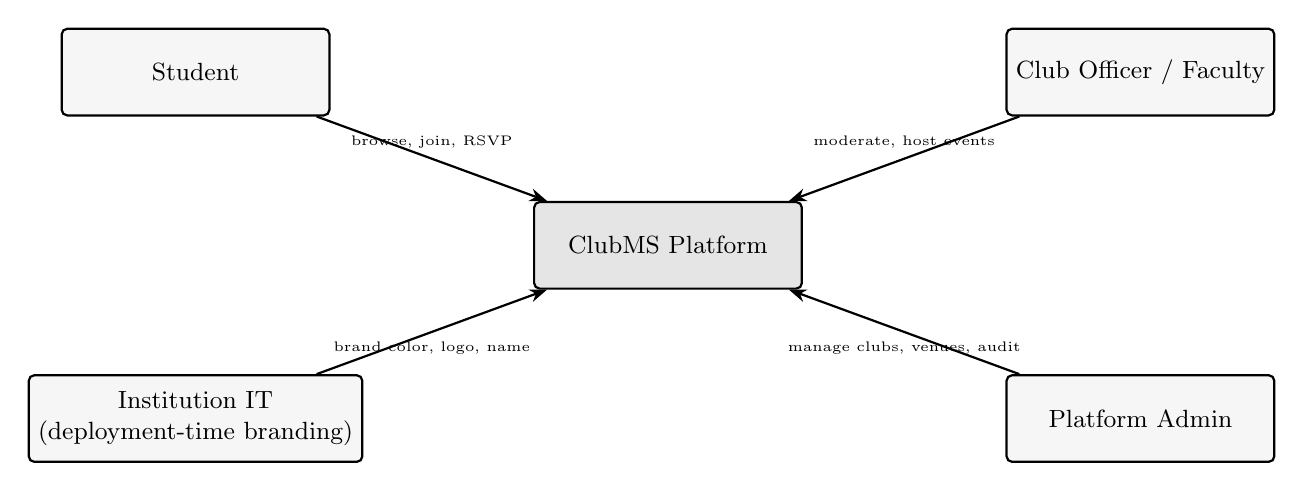
\begin{tikzpicture}
\node[hl] (core) at (0,0) {ClubMS Platform};
\node[proc] (student) at (-6,2.2) {Student};
\node[proc] (officer) at (6,2.2) {Club Officer / Faculty};
\node[proc] (admin) at (6,-2.2) {Platform Admin};
\node[proc] (deploy) at (-6,-2.2) {Institution IT\\(deployment-time branding)};
\draw[arr] (student) -- node[lbl,above]{browse, join, RSVP} (core);
\draw[arr] (officer) -- node[lbl,above]{moderate, host events} (core);
\draw[arr] (admin) -- node[lbl,below]{manage clubs, venues, audit} (core);
\draw[arr] (deploy) -- node[lbl,below]{brand color, logo, name} (core);
\end{tikzpicture}%
}
\caption{System context diagram showing ClubMS's principal actors}
\label{fig:3.1}
\end{figure}


% #####################################################################
\chapter{System Development}
% #####################################################################

\section{Development Methodology}

ClubMS was developed iteratively rather than through a single up-front design phase, following an approach close to Agile feature-slicing: each iteration delivered a vertically complete slice of functionality (database migration, service logic, route, and corresponding UI) before moving to the next. Table~\ref{tab:4.1} summarizes the major development phases as recorded in the project's version-control history, spanning approximately five months.

\begin{table}[H]
\caption{Development phases and timeline}
\label{tab:4.1}
\centering
\small
\begin{tabularx}{\textwidth}{@{}p{2.6cm}X@{}}
\toprule
Period & Milestone \\
\midrule
Apr. 2026 & Project foundation: Express/Prisma backend skeleton, JWT authentication, initial React shell, routing, and layout. \\
Apr.--May 2026 & Club directory and CRUD, membership lifecycle with role hierarchy, events CRUD with calendar view, seed/deseed tooling, security hardening pass. \\
May 2026 & RSVP, dashboard analytics, accessibility pass, skeleton loading states, file upload with dark-mode support, code splitting, first audit-logging pass, initial automated test suite, CI pipeline. \\
Jun. 2026 & Self-action guards on privileged operations; multi-host events with a dedicated co-host feature. \\
Jul. 2026 & Upload security hardening (magic-byte validation, CSP-locked static serving) and read-retry logic; managed venue directory and admin UI. \\
Aug. 2026 & Consent-based cross-club co-host invitations; multipart registration with student ID and ID-card upload; department-based club join rules; club rules and join-agreement flow; membership position field; final UI and accessibility polish. \\
\bottomrule
\end{tabularx}
\end{table}

\section{System Architecture}

ClubMS follows a three-tier client-server architecture: a React single-page application (SPA) communicates with a stateless Express REST API over JSON, and the API is the sole component that talks to the PostgreSQL database, through Prisma ORM. All three components (database, backend, frontend) are packaged as separate Docker containers orchestrated by Docker Compose. Figure~\ref{fig:4.1} shows the full picture: the client tier, the two containerized service tiers, and the layered request pipeline inside the backend container -- security middleware (Helmet, CORS, rate limiting), JWT authentication, role-based access control, Zod schema validation, the controller, the service layer where business rules and transactions live, and finally Prisma ORM for database access. The service layer also writes directly to the \texttt{/uploads} volume for validated file storage, bypassing the ORM entirely since uploaded files are not relational data.

\begin{figure}[H]
\centering
\resizebox{\textwidth}{!}{%
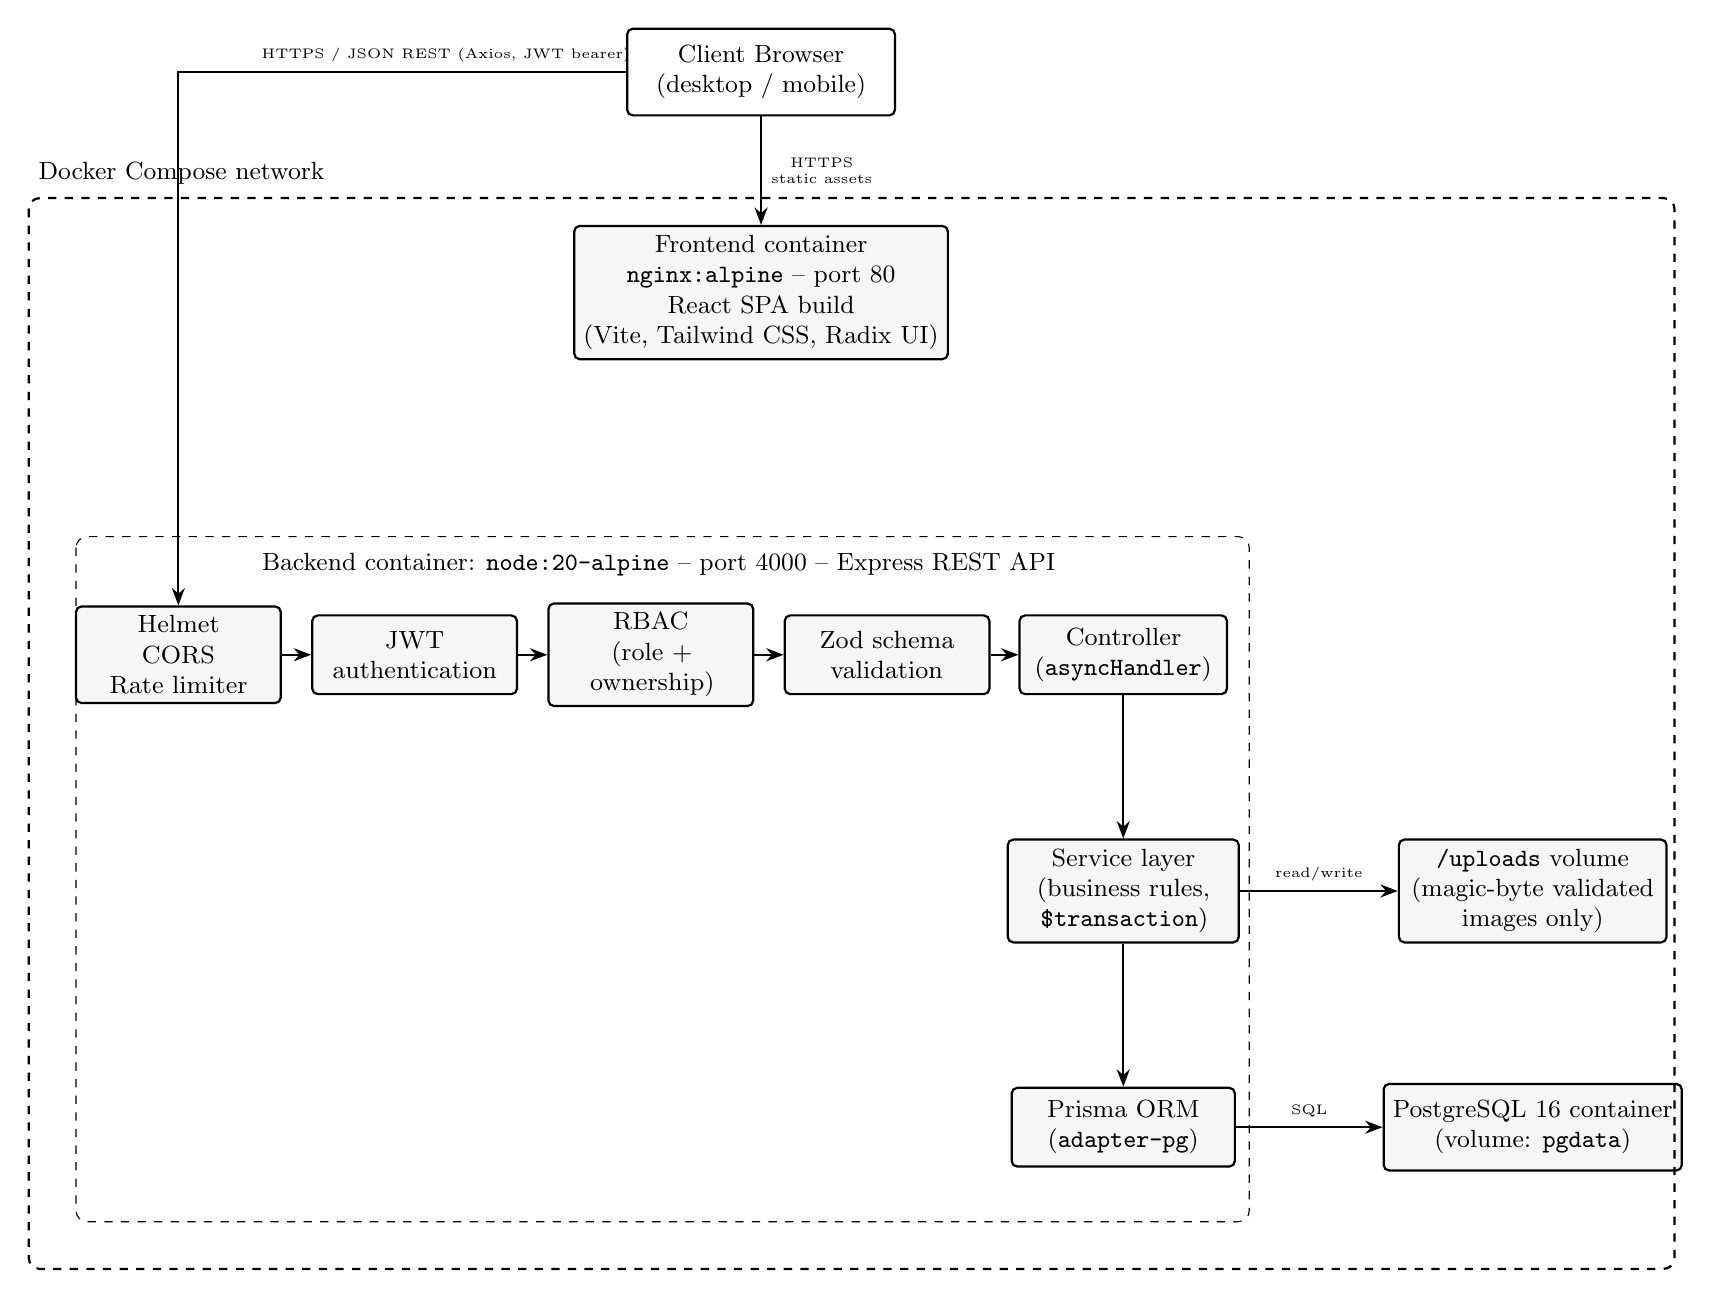
\begin{tikzpicture}
\node[proc, fill=white] (client) at (1,10.6) {Client Browser\\(desktop / mobile)};
\node[proc] (fe) at (1,7.8) {Frontend container\\\texttt{nginx:alpine} -- port 80\\React SPA build\\(Vite, Tailwind CSS, Radix UI)};
\node[ent, text width=2.1cm] (mw1) at (-6.4,3.2) {Helmet\\CORS\\Rate limiter};
\node[ent, text width=2.1cm] (mw2) at (-3.4,3.2) {JWT\\authentication};
\node[ent, text width=2.1cm] (mw3) at (-0.4,3.2) {RBAC\\(role + ownership)};
\node[ent, text width=2.1cm] (mw4) at (2.6,3.2) {Zod schema\\validation};
\node[ent, text width=2.4cm] (ctrl) at (5.6,3.2) {Controller\\(\texttt{asyncHandler})};
\node[ent, text width=2.7cm] (svc) at (5.6,0.2) {Service layer\\(business rules,\\\texttt{\$transaction})};
\node[ent, text width=2.6cm] (prisma) at (5.6,-2.8) {Prisma ORM\\(\texttt{adapter-pg})};
\draw[arr] (mw1) -- (mw2);
\draw[arr] (mw2) -- (mw3);
\draw[arr] (mw3) -- (mw4);
\draw[arr] (mw4) -- (ctrl);
\draw[arr] (ctrl) -- (svc);
\draw[arr] (svc) -- (prisma);
\draw[dashed, rounded corners] (-7.7,4.7) rectangle (7.2,-4.0);
\node[font=\small, align=center] at (-0.3,4.35) {Backend container: \texttt{node:20-alpine} -- port 4000 -- Express REST API};
\node[proc] (up) at (10.8,0.2) {\texttt{/uploads} volume\\(magic-byte validated\\images only)};
\node[proc] (db) at (10.8,-2.8) {PostgreSQL 16 container\\(volume: \texttt{pgdata})};
\draw[arr] (svc) -- node[lbl,above]{read/write} (up);
\draw[arr] (prisma) -- node[lbl,above]{SQL} (db);
\draw[arr] (client) -- node[lbl,right]{HTTPS\\static assets} (fe);
\draw[arr] (client.west) -| (mw1.north);
\node[lbl, above] at (-3.0,10.6) {HTTPS / JSON REST (Axios, JWT bearer)};
\draw[dashed, rounded corners, thick] (-8.3,9.0) rectangle (12.6,-4.6);
\node[font=\small, anchor=south west] at (-8.3,9.05) {Docker Compose network};
\end{tikzpicture}%
}
\caption{Detailed system architecture: client tier, containerized frontend/backend/data tiers, and the backend's layered request pipeline}
\label{fig:4.1}
\end{figure}

\section{Technology Stack}

Table~\ref{tab:4.2} lists the primary technology choices per architectural layer.

\begin{table}[H]
\caption{Technology stack summary}
\label{tab:4.2}
\centering
\small
\begin{tabularx}{\textwidth}{@{}p{2.6cm}X@{}}
\toprule
Layer & Technologies \\
\midrule
Frontend & React 19 [11], Vite 6, React Router 7, Tailwind CSS v4 [18], Radix UI primitives [19], class-variance-authority, Axios, Sonner (toasts), Lucide icons \\
Backend & Node.js, Express 4 [12], Zod schema validation [20], JSON Web Tokens [16], bcryptjs [17], Multer, Helmet, express-rate-limit, Pino structured logging, Swagger/OpenAPI documentation \\
Data layer & PostgreSQL 16 [14], Prisma ORM 7 with the \texttt{@prisma/adapter-pg} driver adapter [13] \\
Testing & Jest, Supertest, Testcontainers (ephemeral PostgreSQL per test run) [21] \\
DevOps & Docker and Docker Compose [15], GitHub Actions CI \\
\bottomrule
\end{tabularx}
\end{table}

\section{Database Design}

The relational schema evolved through eighteen incremental Prisma migrations, from the initial schema in April 2026 to the addition of membership positions in August 2026. The core entities are \texttt{User}, \texttt{Club}, \texttt{ClubMembership}, \texttt{Event}, \texttt{EventHost}, \texttt{EventHostInvite}, \texttt{Venue}, \texttt{EventRsvp}, \texttt{Announcement}, and \texttt{AuditLog}. Figure~\ref{fig:4.2} shows a simplified entity-relationship diagram of the core scheduling and membership entities, drawn in Chen notation: rectangles denote entity sets, diamonds denote named relationship sets, and ovals denote attributes (underlined = primary key, \texttt{...Id} = foreign key), with each edge annotated with its cardinality. The four join tables (\texttt{ClubMembership}, \texttt{EventHost}, \texttt{EventHostInvite}, \texttt{EventRsvp}) appear as associative entities at the many side of their access paths, exactly as they are materialized in the relational schema. \texttt{Announcement} and \texttt{AuditLog} (each a straightforward one-to-many child of \texttt{Club} and/or \texttt{User}) are omitted from the diagram for clarity and are described in Table~\ref{tab:4.3} instead.

\begin{figure}[H]
\centering
\resizebox{\textwidth}{!}{%
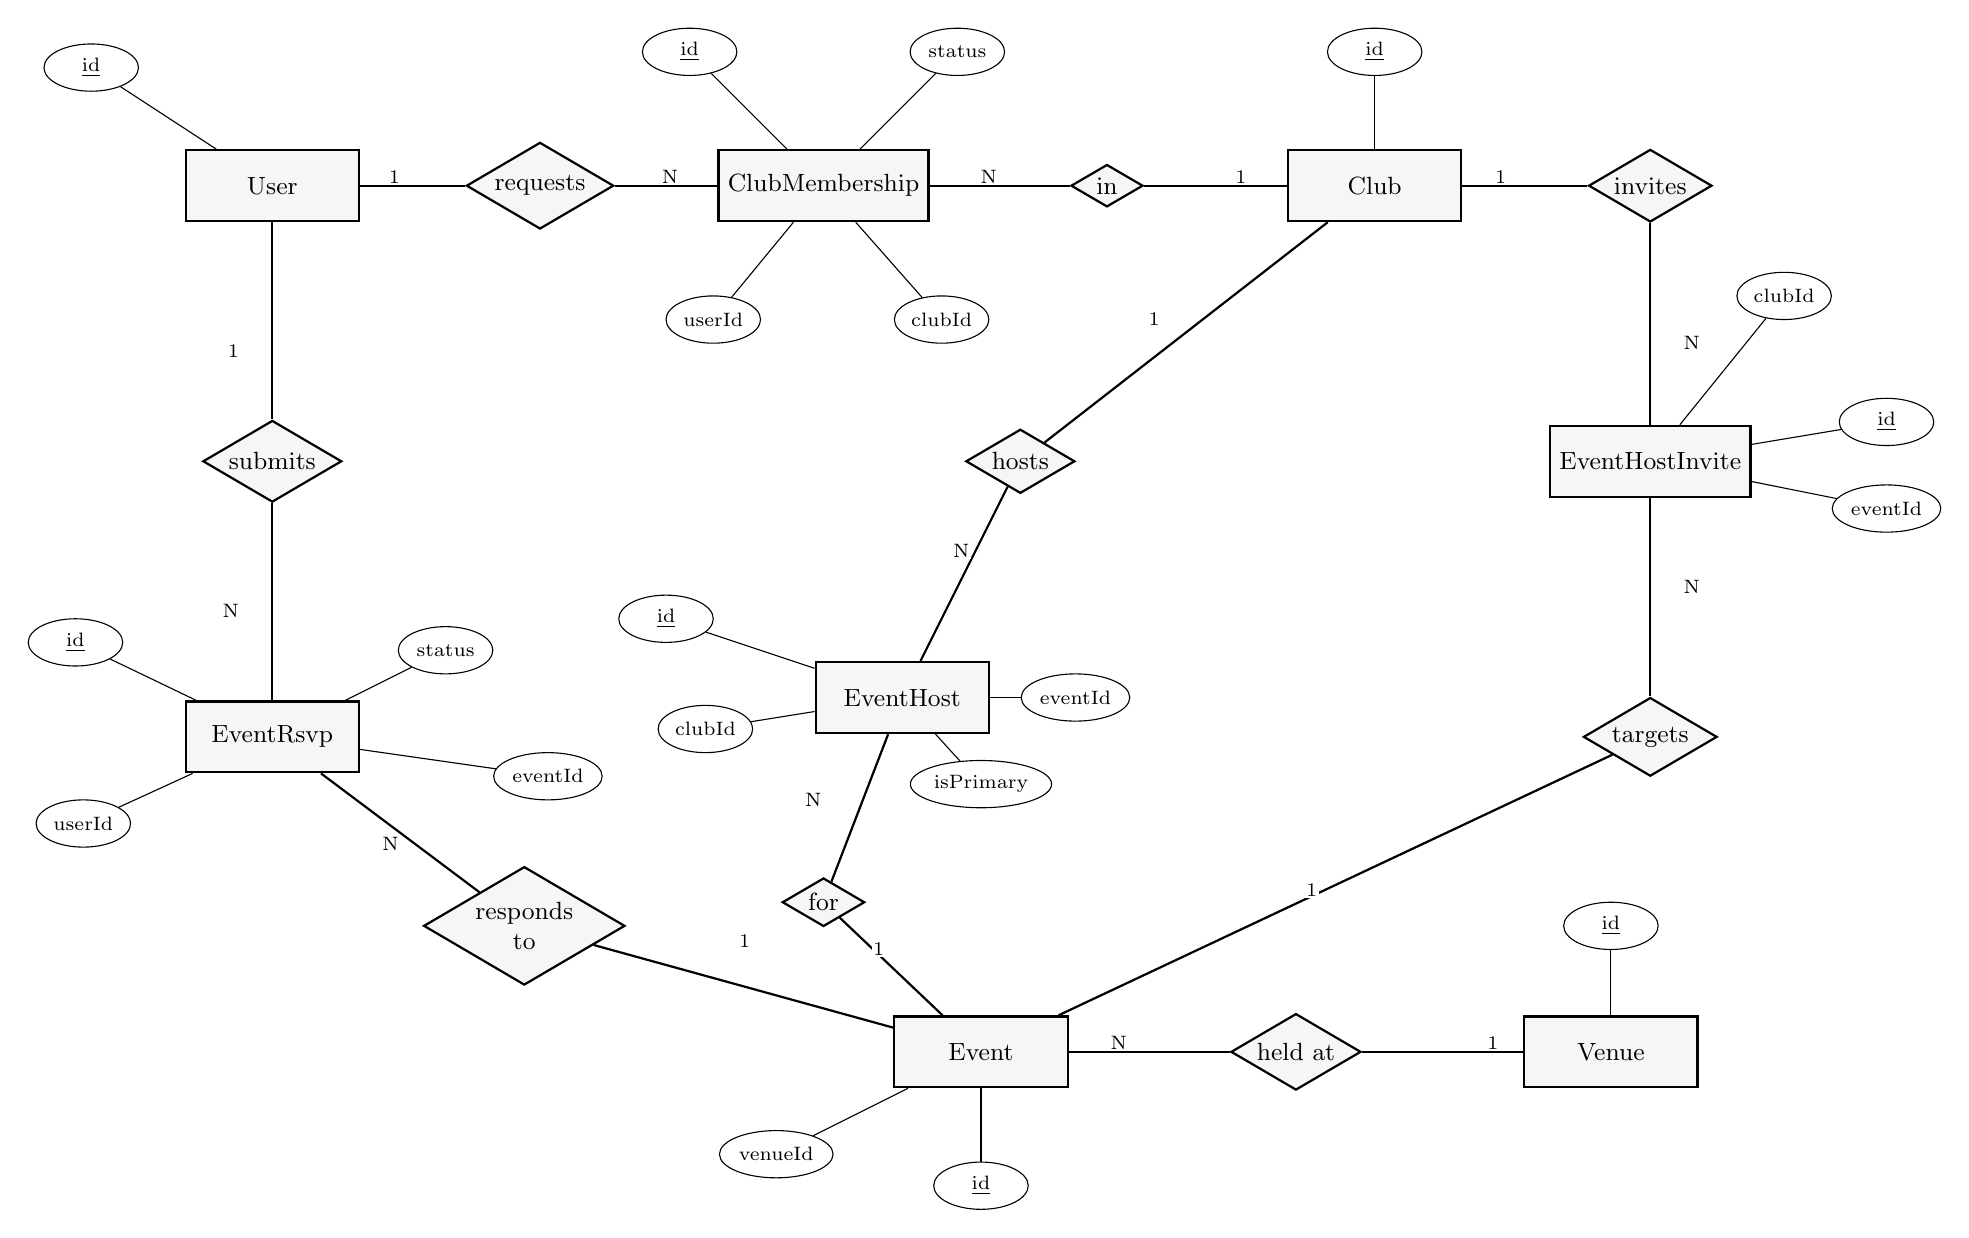
\begin{tikzpicture}[
  ent/.style={draw, thick, rectangle, align=center, minimum width=2.2cm, minimum height=0.9cm, font=\small, fill=gray!7},
  rel/.style={draw, thick, diamond, aspect=1.7, align=center, inner sep=1.5pt, font=\small, fill=gray!7},
  attr/.style={draw, thin, ellipse, align=center, inner sep=1pt, minimum width=1.2cm, minimum height=0.6cm, font=\scriptsize, fill=white},
  ln/.style={thick},
  card/.style={font=\scriptsize, fill=white, inner sep=0.5pt}
]

% ---- Entities
\node[ent] (user)   at (0,11)    {User};
\node[ent] (member) at (7,11)    {ClubMembership};
\node[ent] (club)   at (14,11)   {Club};
\node[ent] (rsvp)   at (0,4)     {EventRsvp};
\node[ent] (host)   at (8,4.5)   {EventHost};
\node[ent] (invite) at (17.5,7.5){EventHostInvite};
\node[ent] (event)  at (9,0)     {Event};
\node[ent] (venue)  at (17,0)    {Venue};

% ---- Relationships
\node[rel] (requests) at (3.4,11)  {requests};
\node[rel] (in)       at (10.6,11) {in};
\node[rel] (submits)  at (0,7.5)   {submits};
\node[rel] (responds) at (3.2,1.6) {responds\\ to};
\node[rel] (hosts)    at (9.5,7.5) {hosts};
\node[rel] (forh)     at (7,1.9)   {for};
\node[rel] (invites)  at (17.5,11) {invites};
\node[rel] (targets)  at (17.5,4)  {targets};
\node[rel] (heldat)   at (13,0)    {held at};

% ---- Attributes (underlined = primary key; ...Id = foreign key)
\node[attr] (userid)     at (-2.3,12.5) {\underline{id}};
\node[attr] (memid)      at (5.3,12.7)  {\underline{id}};
\node[attr] (memstatus)  at (8.7,12.7)  {status};
\node[attr] (memuser)    at (5.6,9.3)   {userId};
\node[attr] (memclub)    at (8.5,9.3)   {clubId};
\node[attr] (clubid)     at (14,12.7)   {\underline{id}};
\node[attr] (hostid)     at (5.0,5.5)   {\underline{id}};
\node[attr] (hostclub)   at (5.5,4.1)   {clubId};
\node[attr] (hostevent)  at (10.2,4.5)  {eventId};
\node[attr] (hostprim)   at (9.0,3.4)   {isPrimary};
\node[attr] (invid)      at (20.5,8.0)  {\underline{id}};
\node[attr] (invevent)   at (20.5,6.9)  {eventId};
\node[attr] (invclub)    at (19.2,9.6)  {clubId};
\node[attr] (rsvpid)     at (-2.5,5.2)  {\underline{id}};
\node[attr] (rsvpstat)   at (2.2,5.1)   {status};
\node[attr] (rsvpuser)   at (-2.4,2.9)  {userId};
\node[attr] (rsapevent)  at (3.5,3.5)   {eventId};
\node[attr] (eventid)    at (9,-1.7)    {\underline{id}};
\node[attr] (eventvenue) at (6.4,-1.3)  {venueId};
\node[attr] (venueid)    at (17,1.6)    {\underline{id}};

% ---- Relationship edges (undirected; cardinality at each entity end)
\draw[ln] (user) -- (requests);   \node[card, above] at (1.55,11)   {1};
\draw[ln] (requests) -- (member); \node[card, above] at (5.05,11)   {N};
\draw[ln] (member) -- (in);       \node[card, above] at (9.1,11)    {N};
\draw[ln] (in) -- (club);         \node[card, above] at (12.3,11)   {1};
\draw[ln] (user) -- (submits);    \node[card, left]  at (-0.4,8.9)  {1};
\draw[ln] (submits) -- (rsvp);    \node[card, left]  at (-0.4,5.6)  {N};
\draw[ln] (rsvp) -- (responds);   \node[card, below] at (1.5,2.75)  {N};
\draw[ln] (responds) -- (event);  \node[card, above] at (6.0,1.3)   {1};
\draw[ln] (club) -- (hosts);      \node[card, above] at (11.2,9.2)  {1};
\draw[ln] (hosts) -- (host);      \node[card, above] at (8.75,6.25) {N};
\draw[ln] (host) -- (forh);       \node[card, left]  at (7.0,3.2)   {N};
\draw[ln] (forh) -- (event);      \node[card, above] at (7.7,1.2)   {1};
\draw[ln] (club) -- (invites);    \node[card, above] at (15.6,11)   {1};
\draw[ln] (invites) -- (invite);  \node[card, right] at (17.9,9.0)  {N};
\draw[ln] (invite) -- (targets);  \node[card, right] at (17.9,5.9)  {N};
\draw[ln] (targets) -- (event);   \node[card, above] at (13.2,1.95) {1};
\draw[ln] (event) -- (heldat);    \node[card, above] at (10.75,0)   {N};
\draw[ln] (heldat) -- (venue);    \node[card, above] at (15.5,0)    {1};

% ---- Attribute links
\draw[thin] (userid) -- (user);
\draw[thin] (memid) -- (member);
\draw[thin] (memstatus) -- (member);
\draw[thin] (memuser) -- (member);
\draw[thin] (memclub) -- (member);
\draw[thin] (clubid) -- (club);
\draw[thin] (hostid) -- (host);
\draw[thin] (hostclub) -- (host);
\draw[thin] (hostevent) -- (host);
\draw[thin] (hostprim) -- (host);
\draw[thin] (invid) -- (invite);
\draw[thin] (invevent) -- (invite);
\draw[thin] (invclub) -- (invite);
\draw[thin] (rsvpid) -- (rsvp);
\draw[thin] (rsvpstat) -- (rsvp);
\draw[thin] (rsvpuser) -- (rsvp);
\draw[thin] (rsapevent) -- (rsvp);
\draw[thin] (eventid) -- (event);
\draw[thin] (eventvenue) -- (event);
\draw[thin] (venueid) -- (venue);
\end{tikzpicture}%
}
\caption{Simplified entity-relationship diagram of the core ClubMS data model}
\label{fig:4.2}
\end{figure}

\begin{table}[H]
\caption{Core data model entities}
\label{tab:4.3}
\centering
\small
\begin{tabularx}{\textwidth}{@{}p{2.6cm}X@{}}
\toprule
Entity & Description \\
\midrule
User & Account record: email, hashed password, role (Student/Club Admin/Faculty/Platform Admin), name, phone, student ID, ID-card image URL, and optional department/home-district. \\
Club & Name, category, logo, description, rules text, and department-based join-rule configuration (mode: all/allow-list/block-list). \\
ClubMembership & Join record between a User and a Club: status (Pending/Active/Alumni/Rejected), member role (Member/Officer), and an optional position title. Unique per (user, club). \\
Event & Title, description, start/end time, venue snapshot, optional foreign key to a managed Venue, banner image, and tags. \\
EventHost & Join table recording which clubs host an event; exactly one row per event has \texttt{isPrimary = true}. \\
EventHostInvite & Pending, not-yet-accepted co-host invitation between an Event and a Club; deleted on accept (converted into an \texttt{EventHost} row) or on reject/cancel. \\
Venue & Reusable, named location that can be attached to events for filtering. \\
EventRsvp & A user's RSVP status (Going/Maybe/Not Going) for an event; unique per (event, user). \\
Announcement & Club-scoped message, optionally pinned, authored by an officer. \\
AuditLog & Immutable record of an administrative action: actor, action name, target type/ID, JSON metadata, and IP address. \\
\bottomrule
\end{tabularx}
\end{table}

Two design decisions in the schema are worth highlighting. First, \texttt{Event} has no direct \texttt{clubId} column; instead, the \texttt{EventHost} join table is the single source of truth for which clubs host an event, which is what makes multi-club co-hosting possible without duplicating events. Second, \texttt{EventHostInvite} deliberately stores only \emph{pending} invitations rather than a status column on \texttt{EventHost} itself, so that authorization logic which queries \texttt{EventHost} (for example, ``is this user an officer of a hosting club'') never has to filter out unaccepted invitations -- an un-accepted invite simply does not exist as a host relationship yet.

\section{API Design}

The API follows conventional REST semantics under the \texttt{/api} prefix, documented interactively through Swagger/OpenAPI at \texttt{/api/docs}. List endpoints return a consistent paginated envelope, \texttt{\{ items, total, page, limit, totalPages \}}, and accept \texttt{page}, \texttt{limit}, and (where applicable) \texttt{search} query parameters. Table~\ref{tab:4.4} lists a representative subset of the full endpoint surface.

\begin{table}[H]
\caption{Representative API endpoints}
\label{tab:4.4}
\centering
\small
\begin{tabularx}{\textwidth}{@{}p{1.3cm}p{4.6cm}X@{}}
\toprule
Method & Path & Purpose \\
\midrule
POST & \url{/api/auth/register} & Multipart registration with ID-card upload \\
POST & \url{/api/auth/login} & Authenticate and receive a JWT \\
GET & \url{/api/clubs} & Paginated, searchable club directory \\
POST & \url{/api/clubs/:clubId/join} & Request membership in a club \\
PATCH & \url{/api/clubs/:clubId/members/:userId/promote} & Promote a member to officer \\
POST & \url{/api/events/:id/cohost-invites} & Invite another club to co-host an event \\
POST & \url{/api/cohost-invites/:id/accept} & Accept an incoming co-host invitation \\
PUT & \url{/api/events/:id/rsvp} & Set the caller's RSVP status for an event \\
GET & \url{/api/events/:id/rsvps} & List (officer-only) RSVPs for an event \\
GET & \url{/api/audit-logs} & Paginated, filterable audit trail (Platform Admin only) \\
POST & \url{/api/upload} & Validate and store an image, returning its URL \\
\bottomrule
\end{tabularx}
\end{table}

\section{Authentication and Authorization}

\subsection{Authentication Flow}
Authentication uses stateless JSON Web Tokens [16]. On login, the server verifies the submitted password against a bcrypt hash [17] and, on success, signs a 24-hour token containing the user's ID, email, and role. The client attaches this token as a Bearer credential on every subsequent request; middleware verifies the signature and expiry before attaching the decoded identity to the request object. Figure~\ref{fig:4.3} illustrates this flow.

\begin{figure}[H]
\centering
\resizebox{\textwidth}{!}{%
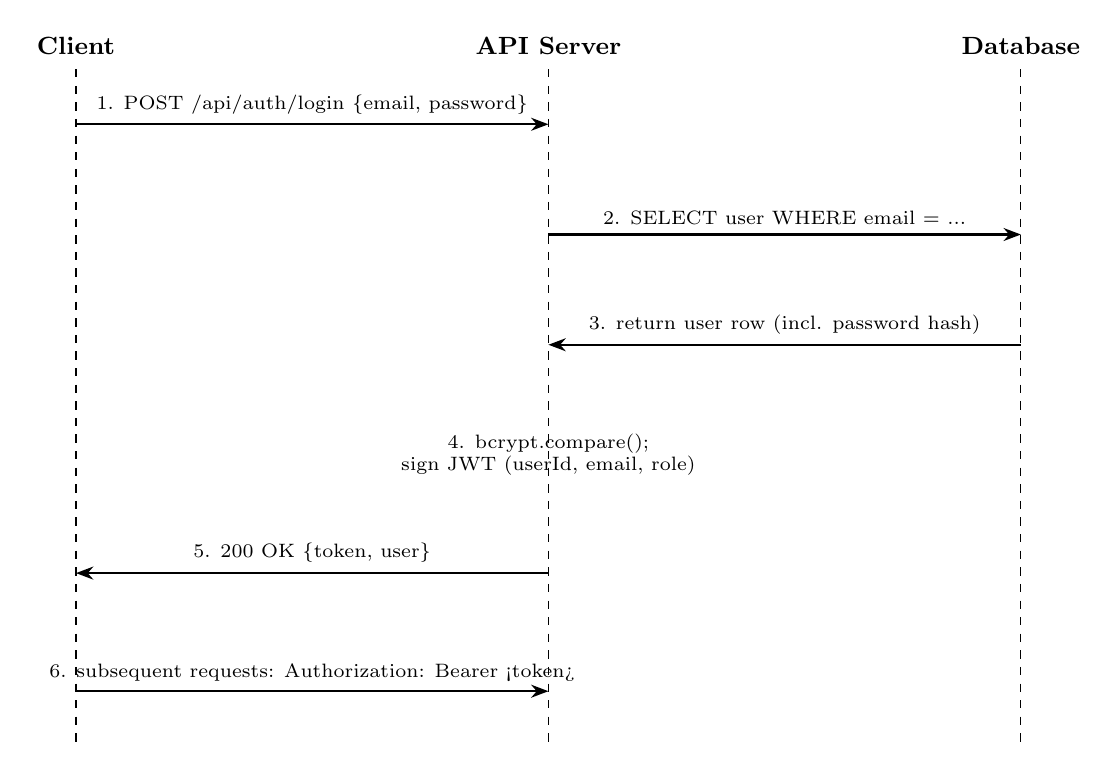
\begin{tikzpicture}[lbl/.append style={font=\scriptsize}]
\node[font=\bfseries\small] (c) at (0,8) {Client};
\node[font=\bfseries\small] (a) at (6,8) {API Server};
\node[font=\bfseries\small] (d) at (12,8) {Database};
\draw[dashed] (0,7.7) -- (0,-0.9);
\draw[dashed] (6,7.7) -- (6,-0.9);
\draw[dashed] (12,7.7) -- (12,-0.9);

\draw[arr] (0,7.0) -- node[lbl,above]{1. POST /api/auth/login \{email, password\}} (6,7.0);
\draw[arr] (6,5.6) -- node[lbl,above]{2. SELECT user WHERE email = ...} (12,5.6);
\draw[arr] (12,4.2) -- node[lbl,above]{3. return user row (incl. password hash)} (6,4.2);
\node[lbl, align=center] at (6,2.8) {4. bcrypt.compare();\\sign JWT (userId, email, role)};
\draw[arr] (6,1.3) -- node[lbl,above]{5. 200 OK \{token, user\}} (0,1.3);
\draw[arr] (0,-0.2) -- node[lbl,above]{6. subsequent requests: Authorization: Bearer <token>} (6,-0.2);
\end{tikzpicture}%
}
\caption{Login and authenticated request sequence}
\label{fig:4.3}
\end{figure}

\subsection{Authorization Model}
Authorization is enforced in two layers. The first is a global role check, \texttt{requireRole(...)}, which consults a static inheritance map so that a Platform Admin automatically satisfies any Club Admin check, and a Faculty user automatically satisfies both Club Admin and Student checks (Figure~\ref{fig:4.4}, Table~\ref{tab:4.5}). The second is a per-resource ownership check, \texttt{requireClubAdmin}, which verifies that the caller is actually an officer of the specific club referenced by the request -- without this second layer, any Club Admin (of any club) could modify any other club's data.

\begin{figure}[H]
\centering
\resizebox{0.7\textwidth}{!}{%
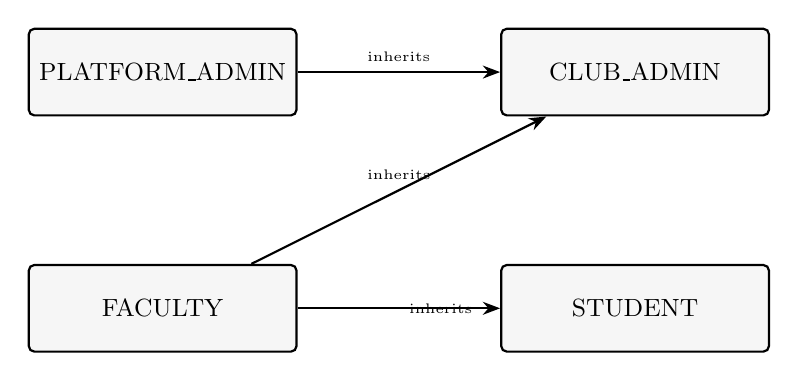
\begin{tikzpicture}
\node[proc] (pa) at (0,3) {PLATFORM\_ADMIN};
\node[proc] (ca) at (6,3) {CLUB\_ADMIN};
\node[proc] (fa) at (0,0) {FACULTY};
\node[proc] (st) at (6,0) {STUDENT};
\draw[arr] (pa) -- node[lbl,above]{inherits} (ca);
\draw[arr] (fa) -- node[lbl,above]{inherits} (ca);
\draw[arr] (fa) -- node[lbl,right]{inherits} (st);
\end{tikzpicture}%
}
\caption{Role inheritance hierarchy}
\label{fig:4.4}
\end{figure}

\begin{table}[H]
\caption{Role inheritance map}
\label{tab:4.5}
\centering
\small
\begin{tabularx}{\textwidth}{@{}>{\RaggedRight\arraybackslash}p{4cm}X@{}}
\toprule
Assigned role & Satisfies role checks for \\
\midrule
PLATFORM\_ADMIN & PLATFORM\_ADMIN, CLUB\_ADMIN \\
FACULTY & FACULTY, CLUB\_ADMIN, STUDENT \\
CLUB\_ADMIN & CLUB\_ADMIN \\
STUDENT & STUDENT \\
\bottomrule
\end{tabularx}
\end{table}

This design underpins several theoretical foundations of role-based access control on the web [7,8]: roles decouple permission assignment from individual identities, while the additional per-resource check implements the principle of least privilege at the level of an individual club rather than the platform as a whole.

\section{Key Module Implementation}

\subsection{Registration and Secure Uploads}
Registration is a multipart form submission combining text fields (name, email, password, phone, student ID) with an ID-card image file. The uploaded file is never trusted by its declared MIME type or filename extension; instead, its first bytes are inspected to determine the true image format, and the file is persisted under a randomly generated name with an extension derived from that detection. The same validated-upload helper is reused for club logos, event banners, and student ID cards, and the entire \texttt{/uploads} directory is served with a strict \texttt{Content-Security-Policy: default-src 'none'} header so that even a successfully uploaded file can never execute script in the browser.

\subsection{Club and Membership Lifecycle}
A club's join behavior is governed by a \texttt{joinRuleMode} of \texttt{ALL}, \texttt{ALLOW}, or \texttt{BLOCK} combined with a list of departments; \texttt{requestJoin} evaluates this rule, and -- if the club has published rules text -- requires the requester to explicitly agree before the request is created. Membership then moves through \texttt{PENDING} $\rightarrow$ \texttt{ACTIVE}/\texttt{REJECTED}, with a rejected user able to re-apply (which resets the same row to \texttt{PENDING} rather than creating a duplicate). Officers can additionally promote a member to \texttt{OFFICER} (which also elevates the user's global role to \texttt{CLUB\_ADMIN}), demote an officer back to member, mark a member as \texttt{ALUMNI}, or remove a membership outright, with guards that prevent a user from demoting or removing themselves and that block removing the club's only remaining officer.

\subsection{Multi-Club Event Hosting and Co-Host Invitations}
Every event has exactly one primary hosting club and may accumulate co-hosts through a consent-based invitation flow, shown in Figure~\ref{fig:4.5}. An officer of any existing host club may invite another club; an officer of the invited club must explicitly accept before an \texttt{EventHost} row is created, or may reject it, and the inviter may cancel an outstanding invitation. This mirrors the same pending-then-confirmed pattern already used for membership requests, and keeps unaccepted invitations completely invisible to authorization checks that determine who may edit or RSVP to an event.

\begin{figure}[H]
\centering
\resizebox{\textwidth}{!}{%
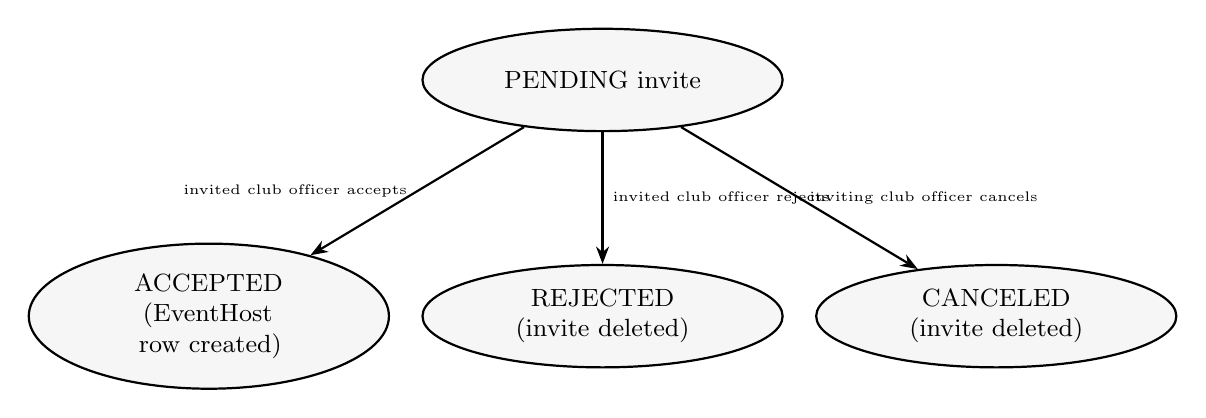
\begin{tikzpicture}
\node[st] (pending) at (5,3) {PENDING invite};
\node[st] (accepted) at (0,0) {ACCEPTED\\(EventHost row created)};
\node[st] (rejected) at (5,0) {REJECTED\\(invite deleted)};
\node[st] (cancelled) at (10,0) {CANCELED\\(invite deleted)};
\draw[arr] (pending) -- node[lbl,left]{invited club officer accepts} (accepted);
\draw[arr] (pending) -- node[lbl,right]{invited club officer rejects} (rejected);
\draw[arr] (pending) -- node[lbl,right]{inviting club officer cancels} (cancelled);
\end{tikzpicture}%
}
\caption{Co-host invitation lifecycle}
\label{fig:4.5}
\end{figure}

\subsection{Audit Logging}
Administrative actions across the clubs, events, and memberships modules are recorded through an Express middleware that patches the response lifecycle to fire an asynchronous, non-blocking write to the \texttt{AuditLog} table after a successful response is sent. This keeps the client-perceived latency unaffected by logging while still producing a durable trail of actor, action, target, and metadata for every privileged mutation, queryable by Platform Admins.

\section{Security Measures}

\begin{table}[H]
\caption{Implemented security measures}
\label{tab:4.6}
\centering
\small
\begin{tabularx}{\textwidth}{@{}p{3.4cm}X@{}}
\toprule
Concern & Mitigation \\
\midrule
Transport / headers & Helmet-applied security headers on every response; strict CSP on the uploads directory \\
Password storage & bcrypt hashing with a per-password salt [17] \\
Session integrity & Signed, expiring JWTs; secret required at startup with no insecure default \\
Cross-origin requests & CORS restricted to the configured frontend origin \\
Brute force / abuse & Rate limiting: 20 requests/15 min on auth endpoints, 100 requests/min generally \\
Injection & All queries parameterized through Prisma; no raw string-concatenated SQL \\
File upload & Magic-byte content validation; extension derived from detected type, never from client input; 5 MB size cap; memory-buffered scan before any disk write \\
Payload size & JSON body size capped at 10 KB \\
Privilege escalation & Two-layer authorization (global role + per-resource ownership); self-action guards on demote/remove \\
Accountability & Immutable audit log of privileged actions [10] \\
\bottomrule
\end{tabularx}
\end{table}

\section{Testing Strategy}

The test suite is split into two layers. Pure unit tests exercise dependency-free utility functions (input validation helpers, the database-retry policy, and the upload magic-byte sniffer) with no I/O. HTTP integration tests build the real Express application (bypassing only \texttt{listen()}) and issue real requests through Supertest against a disposable PostgreSQL 16 instance provisioned per test run by Testcontainers [21], exercising the full middleware chain -- rate limiting, JWT verification, RBAC, Zod validation, controllers, services, and the audit-log middleware -- exactly as it runs in production. The database is reset between tests by truncating all tables, and factory functions build exactly the rows each test needs rather than relying on a shared global seed.

\begin{table}[H]
\caption{Automated test suite composition}
\label{tab:4.7}
\centering
\small
\begin{tabularx}{\textwidth}{@{}p{4.5cm}X@{}}
\toprule
Layer & Coverage \\
\midrule
Unit tests & Validation helpers, database retry policy, upload content-type detection, static file headers \\
Integration tests & Authentication, clubs, memberships, events, RSVP, announcements, co-host invitations, venues, departments, audit log, uploads, dashboard statistics, and platform health \\
Total test cases & 345 automated test cases \\
Continuous Integration & GitHub Actions runs the full suite on every push \\
\bottomrule
\end{tabularx}
\end{table}

\section{Deployment}

The system is packaged as three Docker images orchestrated by a single \texttt{docker-compose.yml}: a PostgreSQL 16 database with a health check and a named volume for durable storage; a Node.js backend image that runs pending Prisma migrations before starting the API server; and a multi-stage frontend image that builds the React application with the institution's branding baked in as build arguments, then serves the static output through Nginx. Figure~\ref{fig:4.7} shows the container topology, and Figure~\ref{fig:4.8} shows the continuous-integration pipeline that validates every change before it reaches deployment.

\begin{figure}[H]
\centering
\resizebox{\textwidth}{!}{%
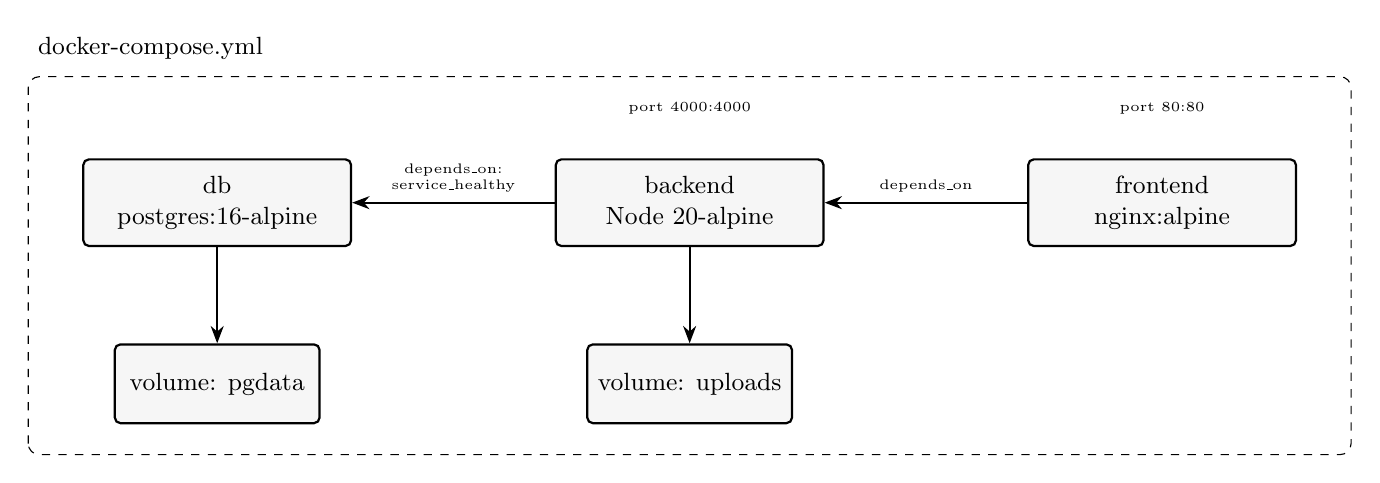
\begin{tikzpicture}
\node[proc] (db) at (0,0) {db\\postgres:16-alpine};
\node[proc] (be) at (6,0) {backend\\Node 20-alpine};
\node[proc] (fe) at (12,0) {frontend\\nginx:alpine};
\node[ent] (v1) at (0,-2.3) {volume: pgdata};
\node[ent] (v2) at (6,-2.3) {volume: uploads};
\draw[arr] (be) -- node[lbl,above]{depends\_on:\\service\_healthy} (db);
\draw[arr] (fe) -- node[lbl,above]{depends\_on} (be);
\draw[arr] (db) -- (v1);
\draw[arr] (be) -- (v2);
\node[lbl] at (12,1.2) {port 80:80};
\node[lbl] at (6,1.2) {port 4000:4000};
\draw[dashed, rounded corners] (-2.4,-3.2) rectangle (14.4,1.6);
\node[font=\small, anchor=south west] at (-2.4,1.7) {docker-compose.yml};
\end{tikzpicture}%
}
\caption{Docker Compose deployment topology}
\label{fig:4.7}
\end{figure}

\begin{figure}[H]
\centering
\resizebox{\textwidth}{!}{%
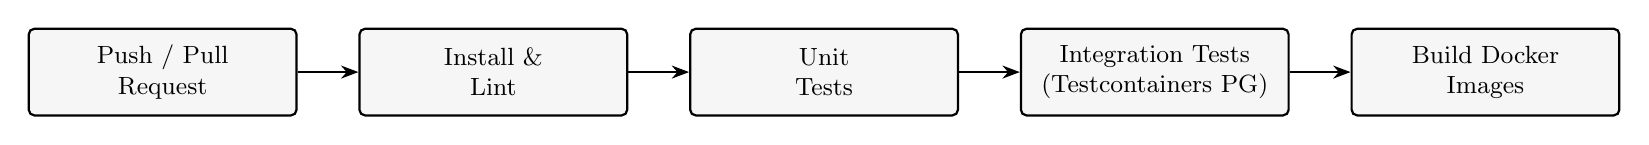
\begin{tikzpicture}
\node[proc] (push) at (0,0) {Push / Pull\\Request};
\node[proc] (install) at (4.2,0) {Install \&\\Lint};
\node[proc] (unit) at (8.4,0) {Unit\\Tests};
\node[proc] (integ) at (12.6,0) {Integration Tests\\(Testcontainers PG)};
\node[proc] (build) at (16.8,0) {Build Docker\\Images};
\draw[arr] (push) -- (install);
\draw[arr] (install) -- (unit);
\draw[arr] (unit) -- (integ);
\draw[arr] (integ) -- (build);
\end{tikzpicture}%
}
\caption{Continuous integration pipeline (GitHub Actions)}
\label{fig:4.8}
\end{figure}


% #####################################################################
\chapter{Results and Discussion}
% #####################################################################

\section{Overview}

This chapter presents the delivered application organized by functional area, with a placeholder for a representative screenshot at each point. Figures should be captured from a running deployment (seeded with the sample data described in the project's seeding guide) and inserted in place of each boxed placeholder.

\section{Authentication and Onboarding}

\ScreenshotFigure{Registration-form.png}{Registration form with student ID and ID-card upload}{fig:5.1}

Figure~\ref{fig:5.1} shows the registration form. New users register with their institutional details and a scanned ID card; the system rejects duplicate emails and student IDs at submission time and shows inline validation errors sourced directly from the backend's Zod schemas.

\section{Role-Based Dashboards}

\ScreenshotFigure{Student-dashboard.png}{Student dashboard: joined clubs and upcoming events}{fig:5.2}

Figure~\ref{fig:5.2} shows the student dashboard: a statistics strip of the student's joined clubs and upcoming events, giving a one-glance view of their own activity.

\ScreenshotFigure{Club-admin-dashboard.png}{Club admin dashboard: managed clubs, pending requests, and co-host invites}{fig:5.3}

Figure~\ref{fig:5.3} shows the club admin dashboard: the clubs the officer manages, with quick links into pending requests and the member roster, plus incoming co-host invitations awaiting a response.

\ScreenshotFigure{PlatForm-admin-dashboard.png}{Platform admin dashboard: platform-wide statistics and Manage Clubs access}{fig:5.4}

Figure~\ref{fig:5.4} shows the platform admin dashboard: platform-wide totals (clubs, users, events, pending memberships) with a direct link into the Manage Clubs page. All three dashboards render a role-specific statistics strip and hide sections entirely rather than disabling them for viewers who are not entitled to see that data.

\section{Club Directory and Detail}

\ScreenshotFigure{All-clubs.png}{Club directory: browsable list of all clubs}{fig:5.5}

\ScreenshotFigure{Club-details-page.png}{Club detail page showing roster, announcements, and published rules (member view)}{fig:5.6}

Figure~\ref{fig:5.5} shows the club directory, which lists every club with its category and member count and lets a visitor search and filter before opening a club's detail page. Figure~\ref{fig:5.6} shows the resulting detail page; it reveals the member roster, contact details, and announcements only to active members and officers, while non-members see the club's public description and published rules without any unauthorized data ever leaving the server.

\section{Membership Management}

\ScreenshotFigure{Member-management.png}{Member management: roles, promote/demote, CSV export}{fig:5.7}

Figure~\ref{fig:5.7} shows the member management page. Officers approve or reject pending applicants in bulk, promote members to Officer or demote them back to Member, and export the full roster as a CSV file for offline record-keeping.

\section{Events and RSVP}

\ScreenshotFigure{All-events.png}{Event listing: all upcoming club events}{fig:5.8}

\ScreenshotFigure{Event-details-page.png}{Event detail page with RSVP controls and attendee count}{fig:5.9}

Students browse all upcoming events across clubs (Figure~\ref{fig:5.8}) and then RSVP as Going, Maybe, or Not Going on the event detail page (Figure~\ref{fig:5.9}); the attendee count updates immediately, and officers of any hosting club can additionally view and export the full RSVP list.

\section{Platform Administration}

\ScreenshotFigure{Manage-clubs.png}{Admin: Manage Clubs page}{fig:5.10}

Figure~\ref{fig:5.10} shows the Manage Clubs page. Platform admins create and edit clubs, assign each one a name, category, logo, and brand color, and the same page surfaces every club's join-rule configuration for quick review.

\section{Discussion}

Measured against the objectives set out in Section~1.4, the delivered system covers all eight of them. The schema, evolved through eighteen migrations, models every entity described in Chapter~4, and the RBAC layer combines role inheritance with per-resource ownership checks. The club and membership lifecycle -- department-based eligibility, join agreements, and all -- is implemented and tested end to end, and multi-club events work through the consent-based invitation model described in Section~4.7.3. Uploads are validated by content rather than trusted metadata, and white-labeling comes down to three build-time environment variables. The whole system is backed by 345 automated tests spanning unit and full-stack integration levels, and it ships as a single Docker Compose file.

Compared with the systems reviewed in Chapter~2, ClubMS's advantage is structural rather than a matter of feature count: none of the academic projects documented a per-resource authorization layer, a consent-based cross-club workflow, or an integration suite tested against a real database, and none of the commercial suites can be self-hosted or white-labeled at all.


% #####################################################################
\chapter{Economic Analysis}
% #####################################################################

\section{Purpose of this Analysis}

Because ClubMS is a self-hosted, open codebase produced as an academic project rather than a commercial product with an existing pricing history, the figures in this chapter are illustrative estimates intended to demonstrate the \emph{shape} of the cost-benefit tradeoff -- self-hosted, one-time development effort versus recurring commercial licensing -- rather than audited financial figures. They should be recalibrated with real quotations before being used for an actual procurement decision.

\section{Development Cost Estimate (Assumption)}

Table~\ref{tab:6.1} breaks the observed development effort down by phase (derived from the project's iteration history in Table~\ref{tab:4.1}) and converts it to an illustrative cost in BDT, using an assumed blended day rate of BDT 1{,}500 -- representative of a junior-to-mid-level software developer's rate in the Bangladeshi IT job market.

\begin{table}[H]
\caption{Illustrative development effort and cost estimate (Bangladeshi Taka)}
\label{tab:6.1}
\centering
\small
\begin{tabularx}{\textwidth}{@{}Xccc@{}}
\toprule
Phase & Effort (person-days) & Rate (BDT/day, assumed) & Cost (BDT) \\
\midrule
Foundation, auth, and core CRUD & 12 & 1{,}500 & 18{,}000 \\
Membership and club lifecycle & 8 & 1{,}500 & 12{,}000 \\
Events, RSVP, and co-hosting & 10 & 1{,}500 & 15{,}000 \\
Admin tools, audit log, venues & 7 & 1{,}500 & 10{,}500 \\
UI/UX, accessibility, theming & 8 & 1{,}500 & 12{,}000 \\
Security hardening & 5 & 1{,}500 & 7{,}500 \\
Automated testing and CI/CD & 6 & 1{,}500 & 9{,}000 \\
Deployment packaging and documentation & 4 & 1{,}500 & 6{,}000 \\
\midrule
\textbf{Total} & \textbf{60} & & \textbf{90{,}000} \\
\bottomrule
\end{tabularx}
\end{table}

\section{Operational Cost Comparison}

Table~\ref{tab:6.2} compares the recurring cost profile of self-hosting ClubMS against the general pricing pattern of commercial campus-engagement suites, which are typically licensed on a per-institution or per-student annual basis rather than a flat hosting fee [3].

\begin{table}[H]
\caption{Illustrative recurring cost comparison (order-of-magnitude estimates)}
\label{tab:6.2}
\centering
\small
\begin{tabularx}{\textwidth}{@{}p{3.6cm}XX@{}}
\toprule
Cost driver & Self-hosted ClubMS & Commercial SaaS suite \\
\midrule
Hosting / infrastructure & Small VPS or on-prem server, approx. USD 10--30/month & Included in subscription \\
Software licensing & None (source available; MIT-style internal use) & Annual per-institution or per-student license fee \\
Customization / branding & Free -- environment variables and, if needed, direct code changes & Limited to vendor-exposed theming options \\
Data ownership & Full control; data never leaves institutional infrastructure & Hosted by vendor; export/portability depends on contract \\
Vendor lock-in risk & Low & High \\
Feature breadth (out of the box) & Core club/event/membership workflow & Broad (ticketing, gamification, budgeting, analytics) \\
\bottomrule
\end{tabularx}
\end{table}

\section{Benefit Analysis}

The primary quantifiable benefit of digitizing club administration is officer time saved: bulk approve/reject of pending membership requests and CSV export of rosters and RSVP lists both replace what would otherwise be manual, per-record work. Qualitatively, the platform also reduces the error rate inherent in spreadsheet-based tracking (duplicate join requests are prevented at the database level by a unique constraint), and the audit log gives student-affairs staff a way to answer ``who approved this, and when'' questions that ad hoc tools cannot answer at all.


% #####################################################################
\chapter{Conclusion}
% #####################################################################

\section{Summary}

This project set out to design and build a self-hosted, white-label club management platform that could replace the manual, fragmented processes many university clubs still rely on, without pushing the institution toward a closed, subscription-priced SaaS product. The delivered system, ClubMS, covers the full club and membership lifecycle with department-based eligibility rules, a multi-club event model with consent-based co-host invitations, RSVP tracking, announcements, and a managed venue directory. Underneath that sits a four-role RBAC system combining global and per-resource authorization, secure content-validated file uploads, a full administrative audit trail, and white-label theming configurable at deployment time. All of it is validated by 345 automated tests -- including HTTP-level integration tests run against a real, disposable PostgreSQL database -- and packaged for one-command deployment with Docker Compose. As Chapter~2 showed, none of the five academic/student projects or the commercial suites reviewed combine all of these properties, which is what this project set out to contribute.

\section{Limitations}

\begin{itemize}
\item \textbf{Single-tenant deployment.} One running instance of ClubMS serves exactly one institution; there is no built-in multi-tenant mode for a single deployment to serve several universities with isolated data.
\item \textbf{No native mobile application.} The frontend is a responsive web SPA; there is no dedicated iOS/Android client, although the API could support one.
\item \textbf{No payments or ticketing.} Unlike some commercial suites, ClubMS does not support paid events, dues collection, or budgeting workflows.
\item \textbf{No email or push notifications.} State changes (approval, RSVP reminders, co-host invitations) are visible only when a user next opens the application; there is no outbound notification channel yet.
\item \textbf{No institutional SSO/LDAP integration.} Authentication is self-contained; it does not integrate with an existing university identity provider.
\item \textbf{Free-text department field.} Departments used for join-rule targeting are free text rather than a curated, centrally managed registry, which can lead to near-duplicate entries (e.g., inconsistent capitalization or abbreviation) if not disciplined by administrators.
\end{itemize}

\section{Recommendations and Future Work}

\begin{enumerate}
\item \textbf{Notifications.} Add email and/or in-app push notifications for membership decisions, upcoming RSVP'd events, and co-host invitations.
\item \textbf{Single sign-on.} Support institutional SSO (SAML/OIDC) or LDAP-backed authentication as an alternative to local email/password accounts.
\item \textbf{Multi-tenancy.} Extend the schema and authorization model to allow one deployment to host several independently branded institutions.
\item \textbf{Co-curricular transcript.} Aggregate a student's memberships, officer positions, and event participation into an exportable involvement record, mirroring a feature common in commercial suites [3].
\item \textbf{Native mobile client.} Build a companion mobile application against the existing REST API, prioritizing the student-facing browse/join/RSVP flows.
\item \textbf{Budgeting and ticketing.} Add optional financial workflows (dues, paid event tickets) for clubs and institutions that need them.
\item \textbf{Calendar interoperability.} Support ICS export/subscription so a student's joined-club events appear in their personal calendar application.
\item \textbf{Internationalization.} Externalize UI strings to support multiple languages beyond the current English-only interface.
\end{enumerate}

\begin{table}[H]
\caption{Limitations mapped to recommended future work}
\label{tab:7.1}
\centering
\small
\begin{tabularx}{\textwidth}{@{}p{6.2cm}X@{}}
\toprule
Limitation & Recommended future work \\
\midrule
No notifications & Email / in-app push notifications \\
No SSO/LDAP integration & Institutional SSO or LDAP support \\
Single-tenant deployment & Multi-tenant architecture \\
No involvement transcript & Co-curricular transcript export \\
No native mobile application & Companion mobile client on the existing API \\
No payments/ticketing & Budgeting and paid-event ticketing module \\
\bottomrule
\end{tabularx}
\end{table}


% =====================================================================
% REFERENCES
% =====================================================================
\begin{spacing}{1.0}
\chapter*{REFERENCES}
\addcontentsline{toc}{chapter}{REFERENCES}

\begin{enumerate}[label={[\arabic*]}, leftmargin=2.2em, itemsep=6pt]

\item\label{ref1} S. H. Syd. Amra, ``Online Club Management System for UiTM Terengganu (On-ClubS),'' B.Sc. thesis, Faculty of Computer and Mathematical Sciences, Universiti Teknologi MARA, Jan. 2017.

\item\label{ref2} Y. Ainapure, R. Patil, S. Bhadgaonkar, P. Sawant, and M. Pardesi, ``DYPCETCLUBS -- A Unified Platform for Management of College Clubs,'' \textit{International Journal of Innovative Research in Computer and Communication Engineering}, vol. 13, no. 3, Mar. 2025.

\item\label{ref3} Modern Campus and CampusGroups, ``Student engagement and involvement platforms,'' Modern Campus Involve / CampusGroups product documentation, accessed 2026. [Online]. Available: \url{https://moderncampus.com/products/student-engagement-and-learning-platform} and \url{https://www.readyeducation.com/campusgroups/}

\item\label{ref4} S. Kumar, S. Kumar, S. Chowdary, and E. Murali, ``Club Management System: A MERN Stack-Based Web Application for Event Management in Colleges,'' \textit{International Journal of Innovations in Engineering and Science}, vol. 10, no. 7, Jun. 2025.

\item\label{ref5} K. K. Nath, S. Mohite, S. Dhapate, S. S. Chauhan, and A. Gaikwad, ``College Club Management System -- Digitizing Student Engagement and Organizational Efficiency,'' \textit{Iconic Research and Engineering Journals}, vol. 8, no. 11, pp. 1433--1437, May 2025.

\item\label{ref6} W. Qi, ``Design and Implementation of University Club Management System based on WeChat Applet,'' \textit{Journal of Computing and Electronic Information Management}, 2024.

\item\label{ref7} J. S. Park, R. Sandhu, and G.-J. Ahn, ``Role-Based Access Control on the Web,'' \textit{ACM Transactions on Information and System Security}, vol. 4, no. 1, pp. 37--71, Feb. 2001.

\item\label{ref8} W. A. Jansen, ``A Revised Model for Role-Based Access Control,'' NISTIR 6192, National Institute of Standards and Technology, Jul. 1998.

\item\label{ref9} World Wide Web Consortium (W3C), ``Web Content Accessibility Guidelines (WCAG) 2.1,'' W3C Recommendation, Jun. 2018. [Online]. Available: \url{https://www.w3.org/TR/WCAG21/}

\item\label{ref10} OWASP Foundation, ``OWASP Top 10:2021 -- The Ten Most Critical Web Application Security Risks,'' 2021. [Online]. Available: \url{https://owasp.org/www-project-top-ten/}

\item\label{ref11} Meta Platforms, Inc., ``React Documentation,'' 2026. [Online]. Available: \url{https://react.dev}

\item\label{ref12} OpenJS Foundation, ``Express.js Documentation,'' 2026. [Online]. Available: \url{https://expressjs.com}

\item\label{ref13} Prisma Data, Inc., ``Prisma ORM Documentation,'' 2026. [Online]. Available: \url{https://www.prisma.io/docs}

\item\label{ref14} PostgreSQL Global Development Group, ``PostgreSQL 16 Documentation,'' 2024. [Online]. Available: \url{https://www.postgresql.org/docs/16/}

\item\label{ref15} Docker Inc., ``Docker Documentation,'' 2026. [Online]. Available: \url{https://docs.docker.com}

\item\label{ref16} M. Jones, J. Bradley, and N. Sakimura, ``JSON Web Token (JWT),'' IETF RFC 7519, May 2015.

\item\label{ref17} N. Provos and D. Mazi\`eres, ``A Future-Adaptable Password Scheme,'' in \textit{Proceedings of the USENIX Annual Technical Conference}, 1999.

\item\label{ref18} Tailwind Labs Inc., ``Tailwind CSS Documentation,'' 2026. [Online]. Available: \url{https://tailwindcss.com/docs}

\item\label{ref19} WorkOS, ``Radix UI Primitives Documentation,'' 2026. [Online]. Available: \url{https://www.radix-ui.com}

\item\label{ref20} C. McDonnell, ``Zod: TypeScript-first Schema Validation,'' 2026. [Online]. Available: \url{https://zod.dev}

\item\label{ref21} AtomicJar, Inc., ``Testcontainers Documentation,'' 2026. [Online]. Available: \url{https://testcontainers.com}

\end{enumerate}
\end{spacing}

\end{document}